\section{Edge insertion time}

\paragraph{}
To see the effect of,

\begin{itemize}
    \item Memory allocation
    \item Number of edges already present in the sketch
\end{itemize}

on the speed of the edge operations.

\subsection*{Memory allocation}

\subsubsection{Purpose}

\paragraph{}
To analyze the speed of the edge operations (insertion) with respect to memory allocated for the sketch.

\subsubsection{Results}

\begin{figure}[H]
    \centering 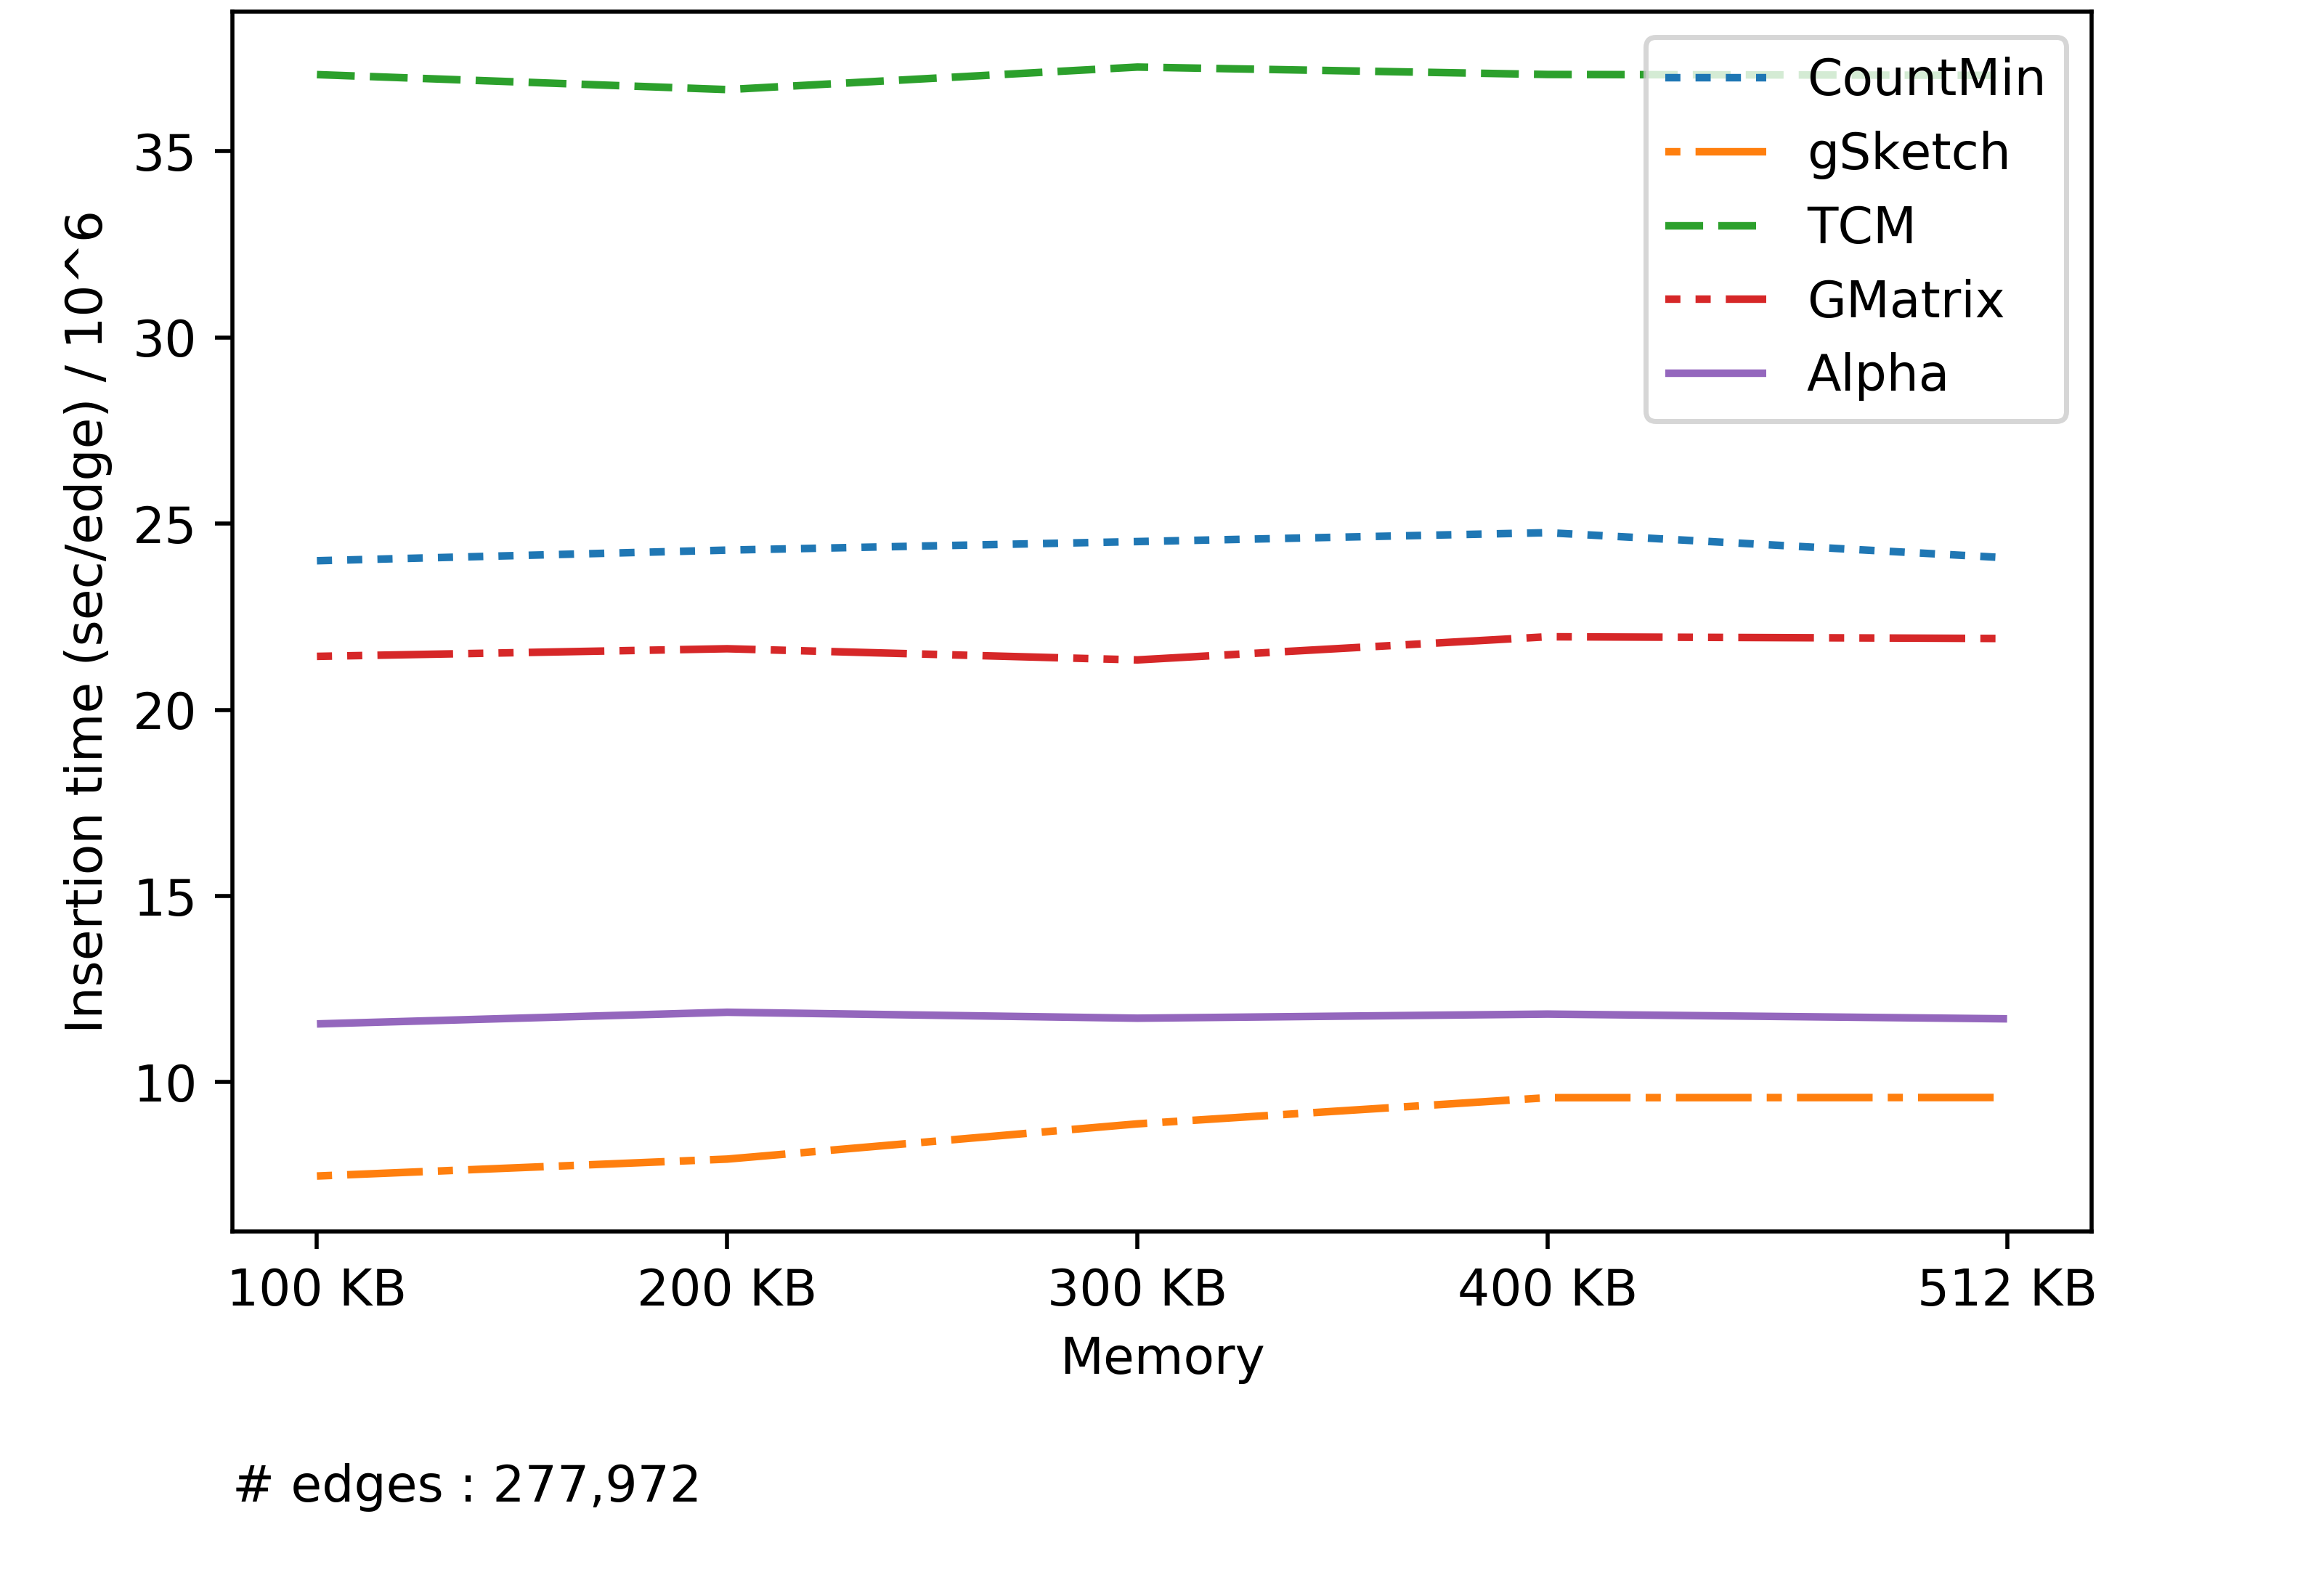
\includegraphics[width=0.85\textwidth]{results/insertion/unicorn-wget-insertiontime1}
    \vspace{-0.5cm}
    \caption{Insertion time per edge vs Memory for unicorn-wget dataset}
    \label{fig:unicorn-wget-insertiontime1}
\end{figure}

\begin{figure}[H]
    \centering 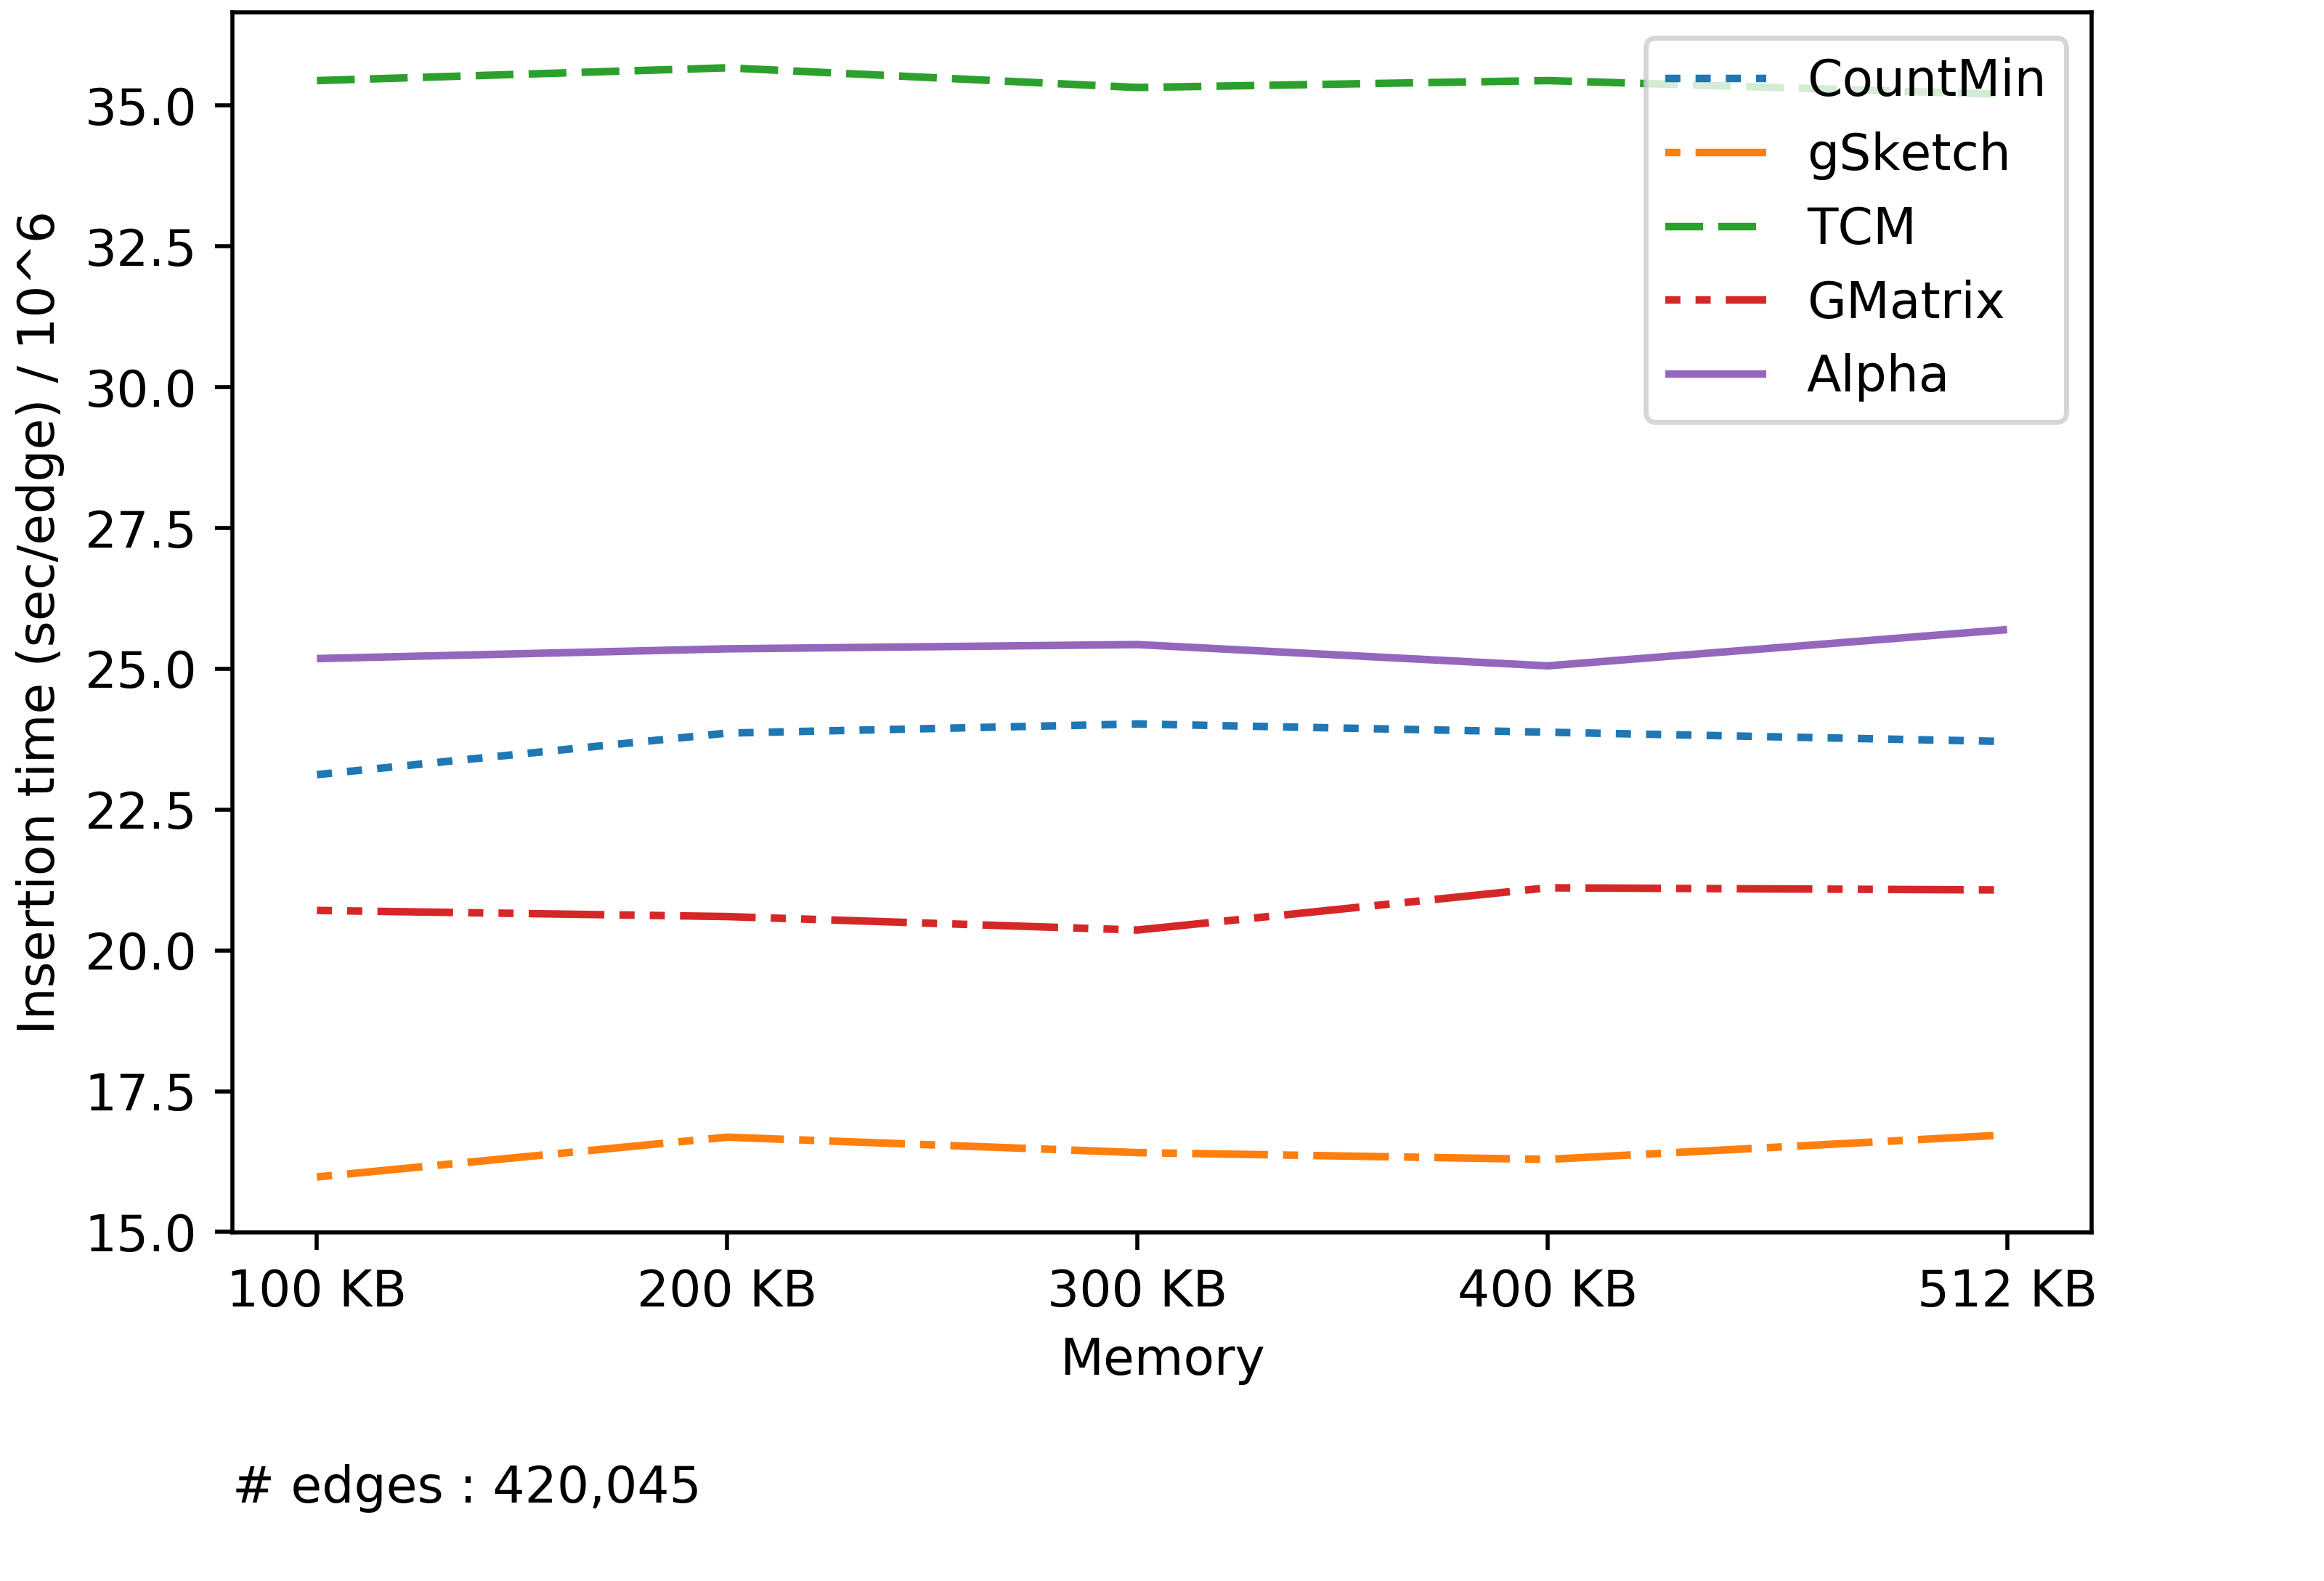
\includegraphics[width=0.85\textwidth]{results/insertion/email-EuAll-insertiontime1}
    \vspace{-0.5cm}
    \caption{Insertion time per edge vs Memory for email-EuAll dataset}
    \label{fig:email-EuAll-insertiontime1}
\end{figure}

\begin{figure}[H]
    \centering 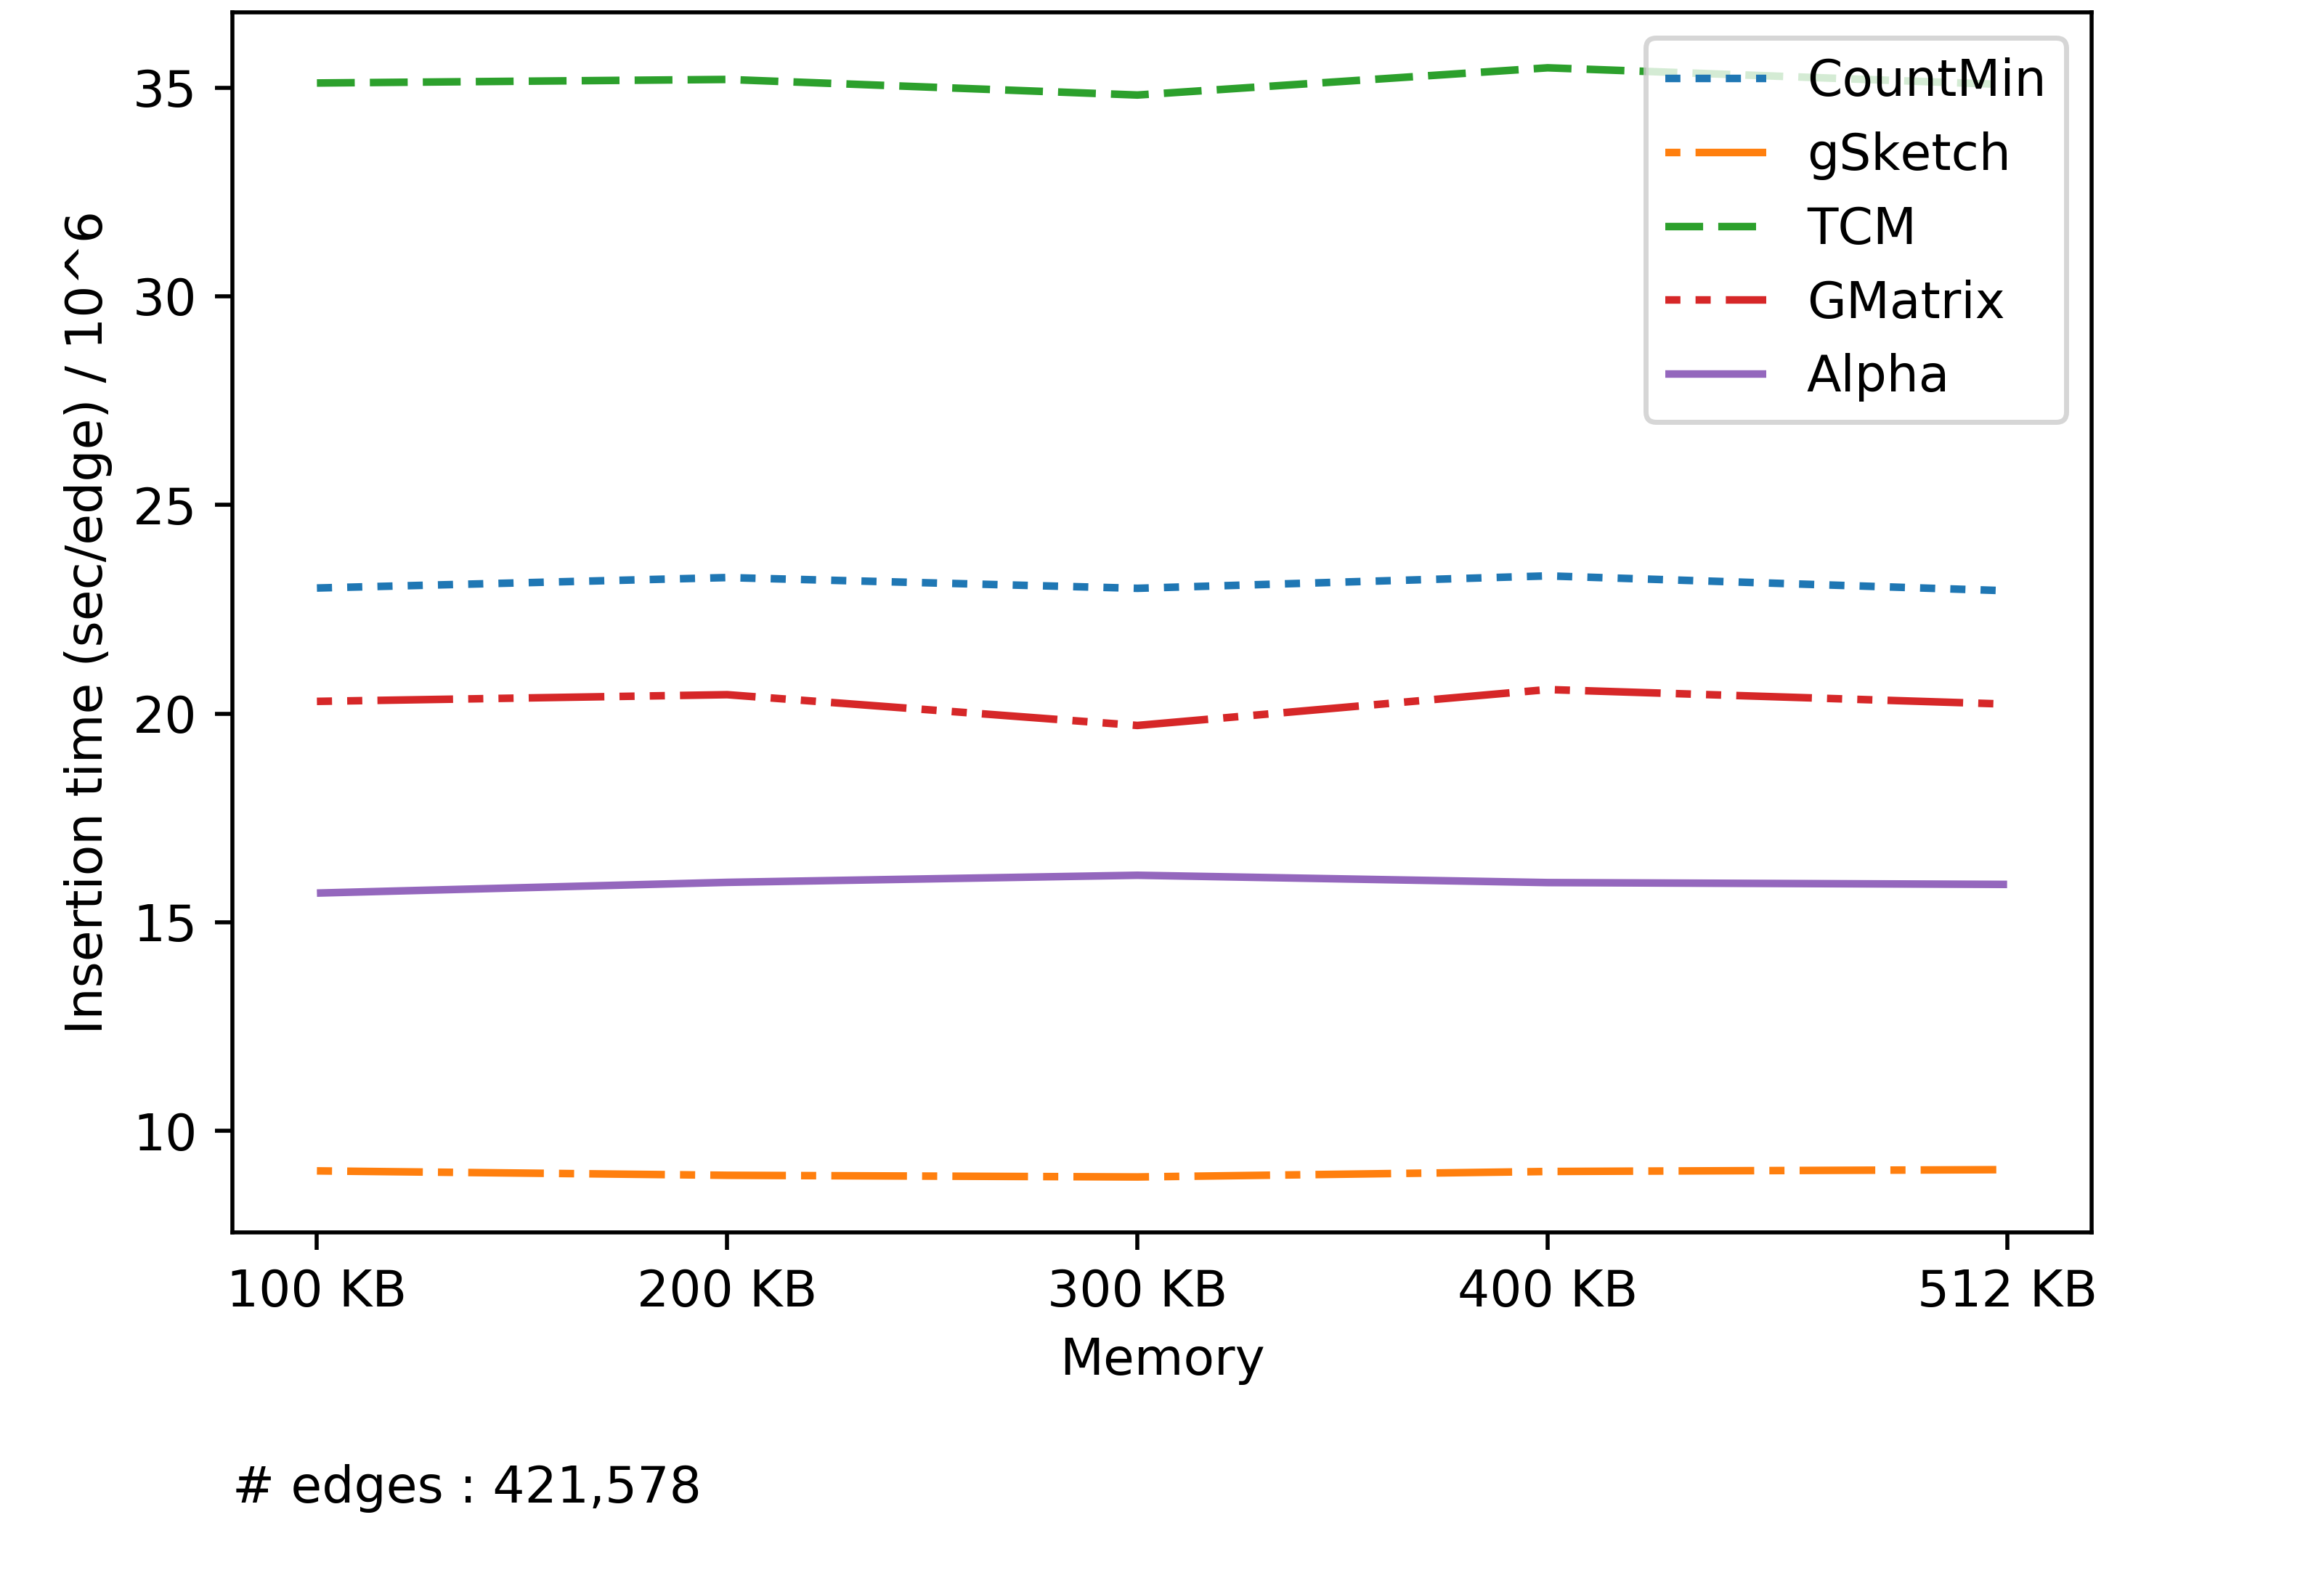
\includegraphics[width=0.85\textwidth]{results/insertion/cit-HepPh-insertiontime1}
    \vspace{-0.5cm}
    \caption{Insertion time per edge vs Memory for cit-HepPh dataset}
    \label{fig:cit-HepPh-insertiontime1}
\end{figure}

\begin{figure}[H]
    \centering 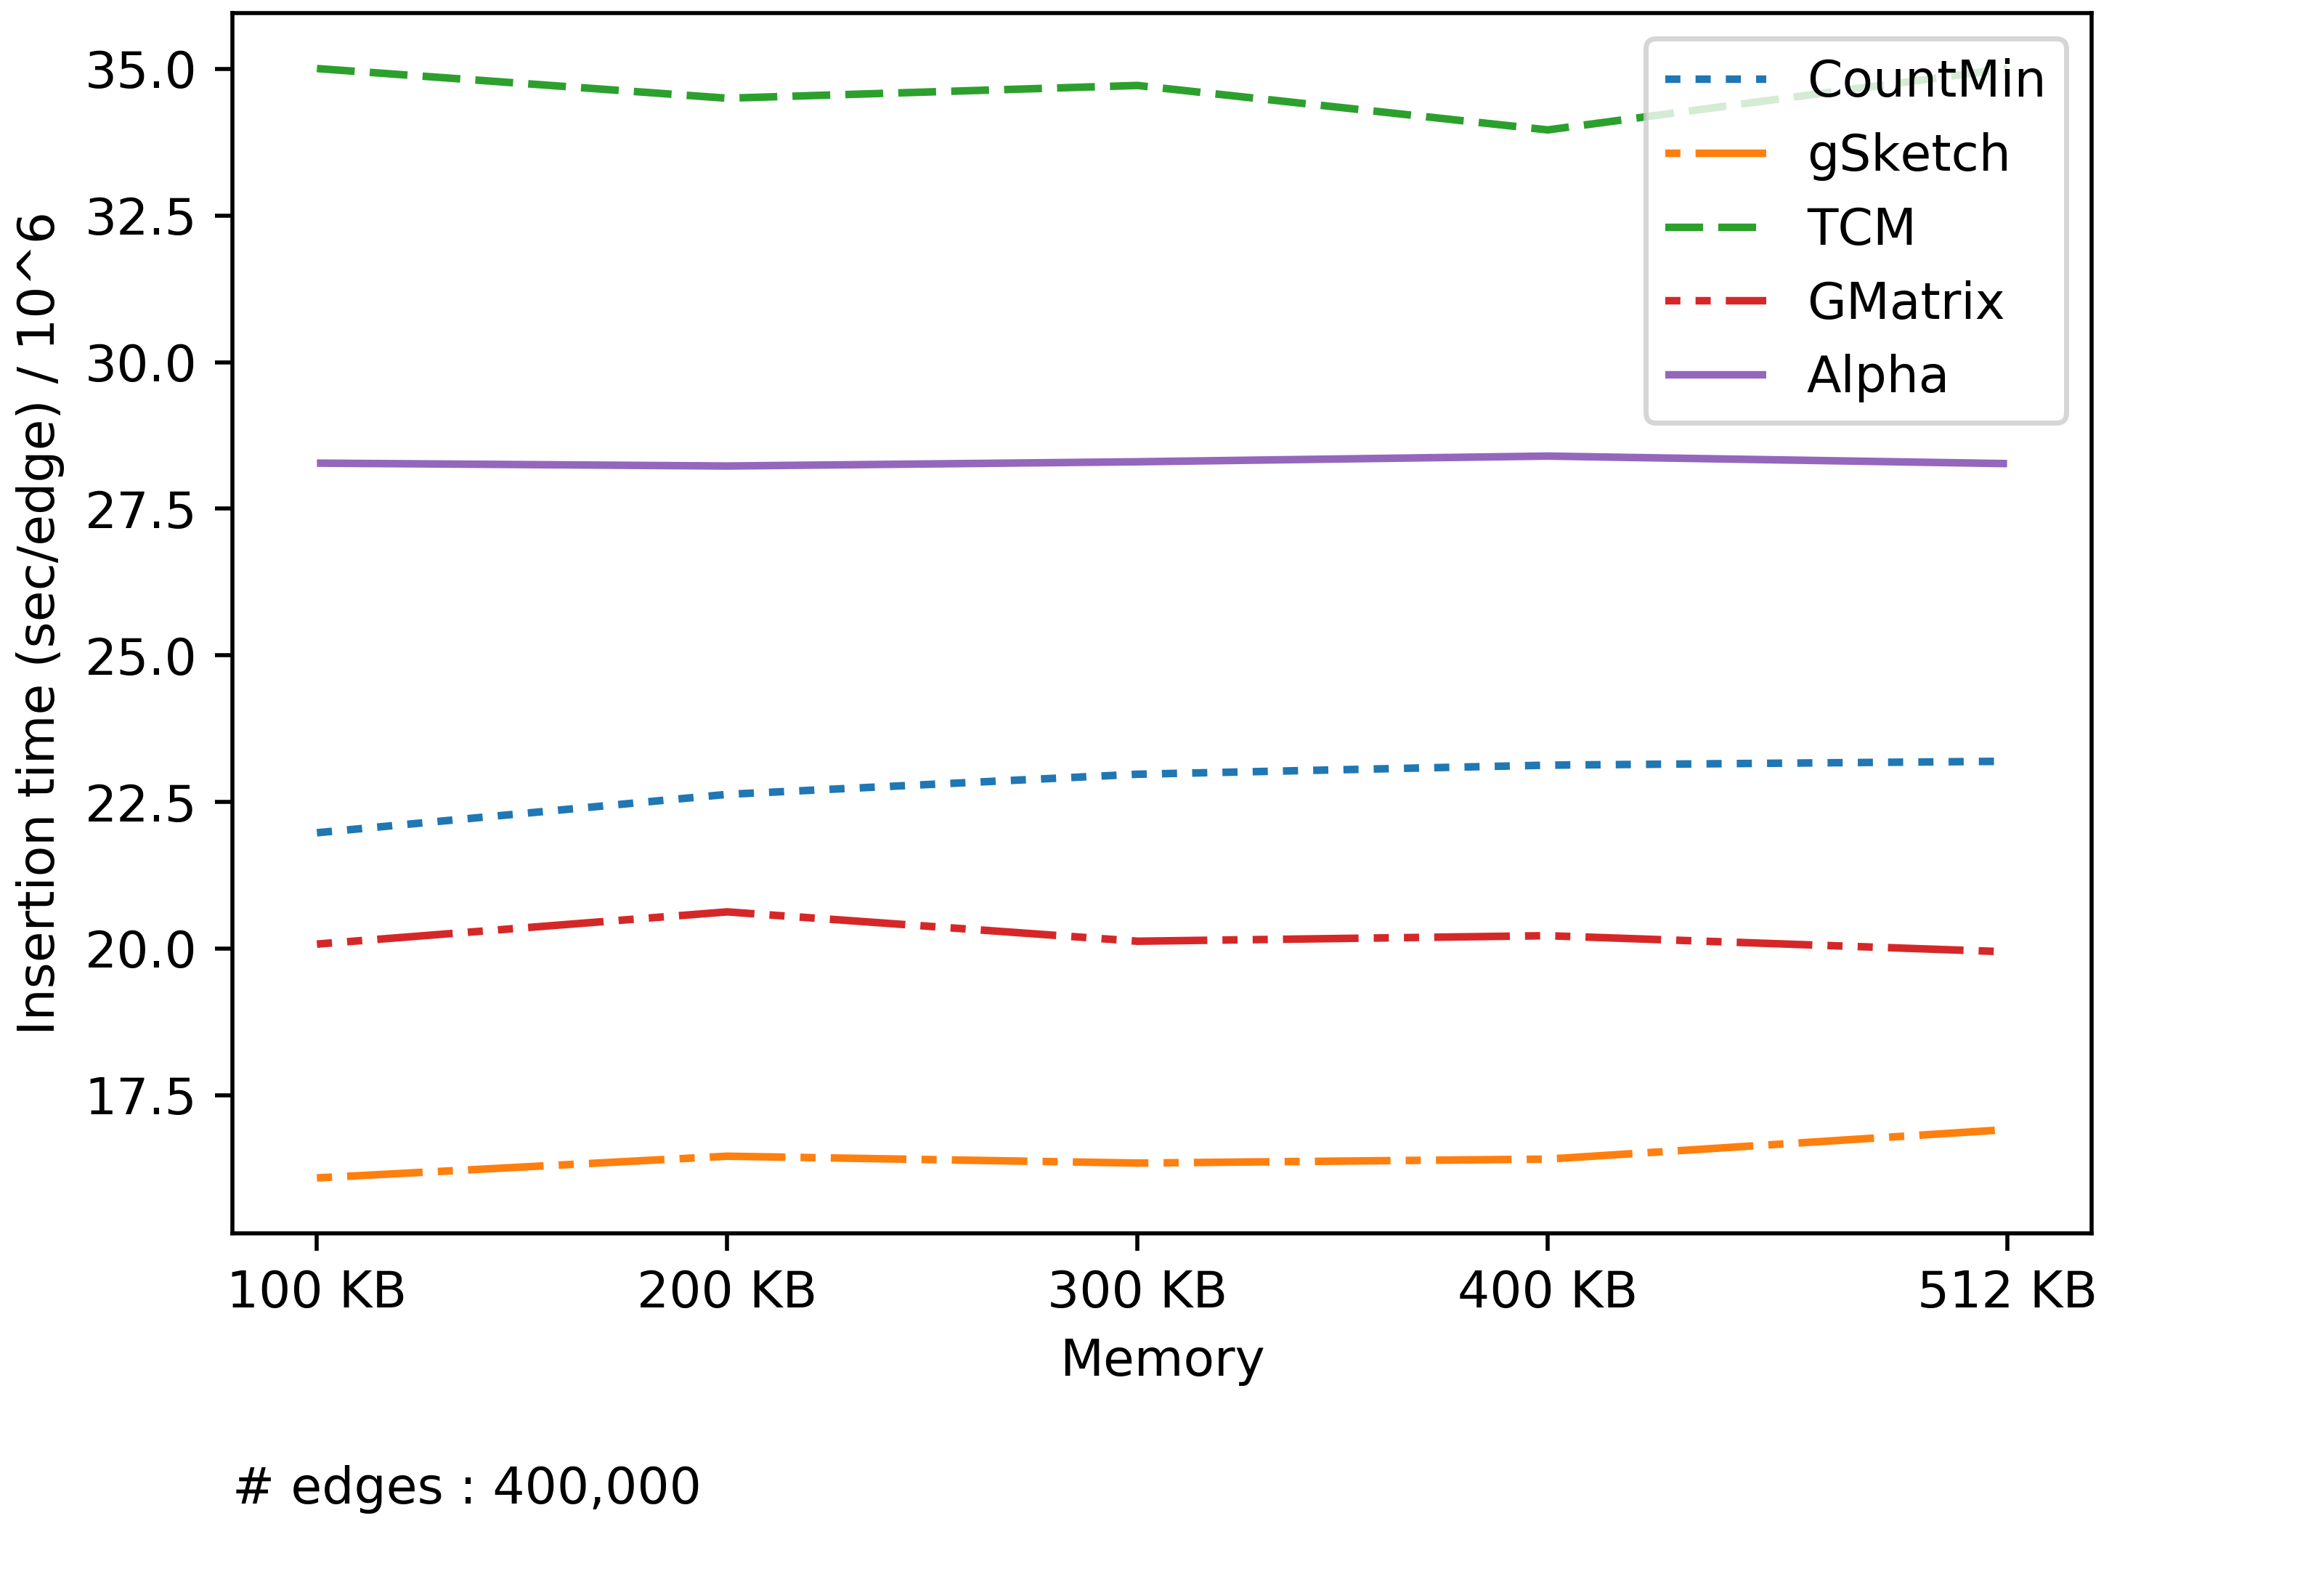
\includegraphics[width=0.85\textwidth]{results/insertion/gen-scale-free-insertiontime1}
    \vspace{-0.5cm}
    \caption{Insertion time per edge vs Memory for gen-scale-free dataset}
    \label{fig:gen-scale-free-insertiontime1}
\end{figure}

\begin{figure}[H]
    \centering 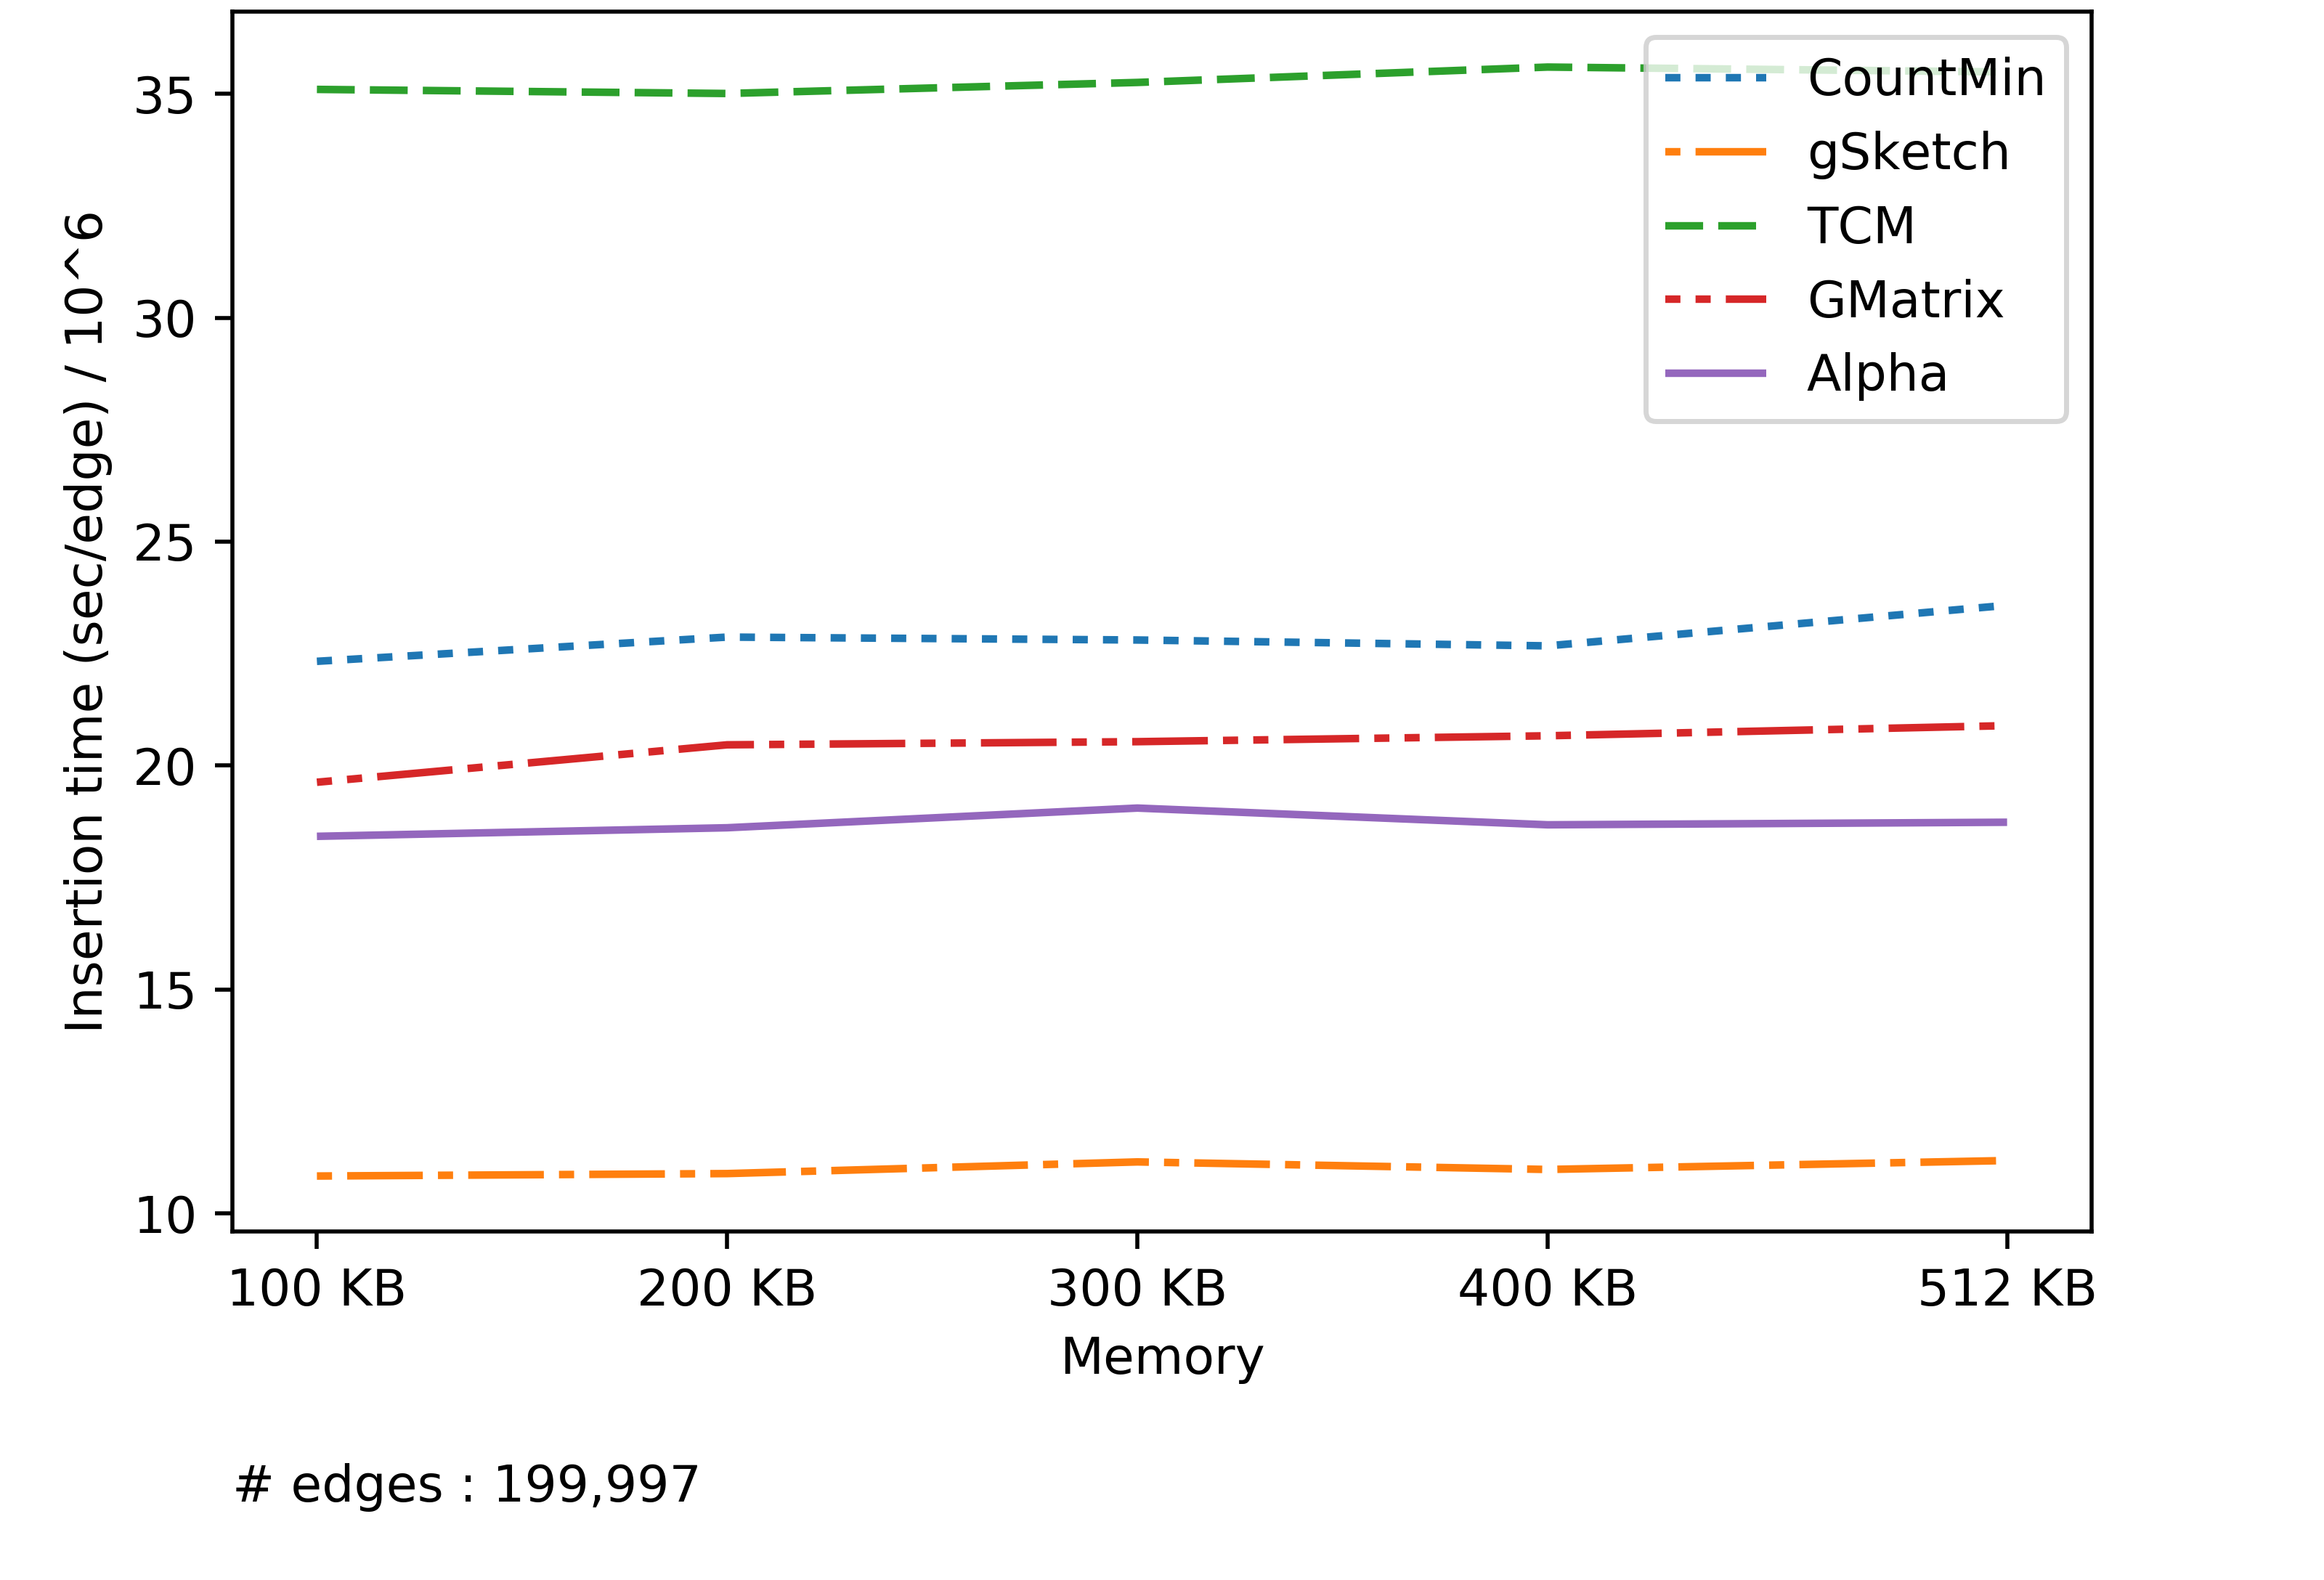
\includegraphics[width=0.85\textwidth]{results/insertion/gen-small-world-insertiontime1}
    \vspace{-0.5cm}
    \caption{Insertion time per edge vs Memory for gen-small-world dataset}
    \label{fig:gen-small-world-insertiontime1}
\end{figure}

\subsubsection{Observations and inferences}

\paragraph{}
The proposed sketch Alpha shows faster speeds of insertion operations on the datasets, unicorn-wget in \autoref{fig:unicorn-wget-insertiontime1}, cit-HepPh in \autoref{fig:cit-HepPh-insertiontime1} and gen-small-world in \autoref{fig:gen-small-world-insertiontime1}. However this is not the case for email-EuAll in \autoref{fig:email-EuAll-insertiontime1} and gen-scale-free in \autoref{fig:gen-scale-free-insertiontime1}.

\paragraph{}
TCM has yielded the slowest insertion speeds despite the type of the dataset while gSketch has achieved the highest speed for all the datasets.

\subsubsection{Conclusion}

\paragraph{}
gSketch is the suitable type of sketching technique in a scenario where the edge operation speeds are critical.

\subsection*{Number of edges already present in the sketch}

\subsubsection{Purpose}

\paragraph{}
To analyze the speed of the edge operations (insertion) with respect to number of edges that is already present in the sketch.

\subsubsection{Results}

\begin{figure}[H]
    \centering 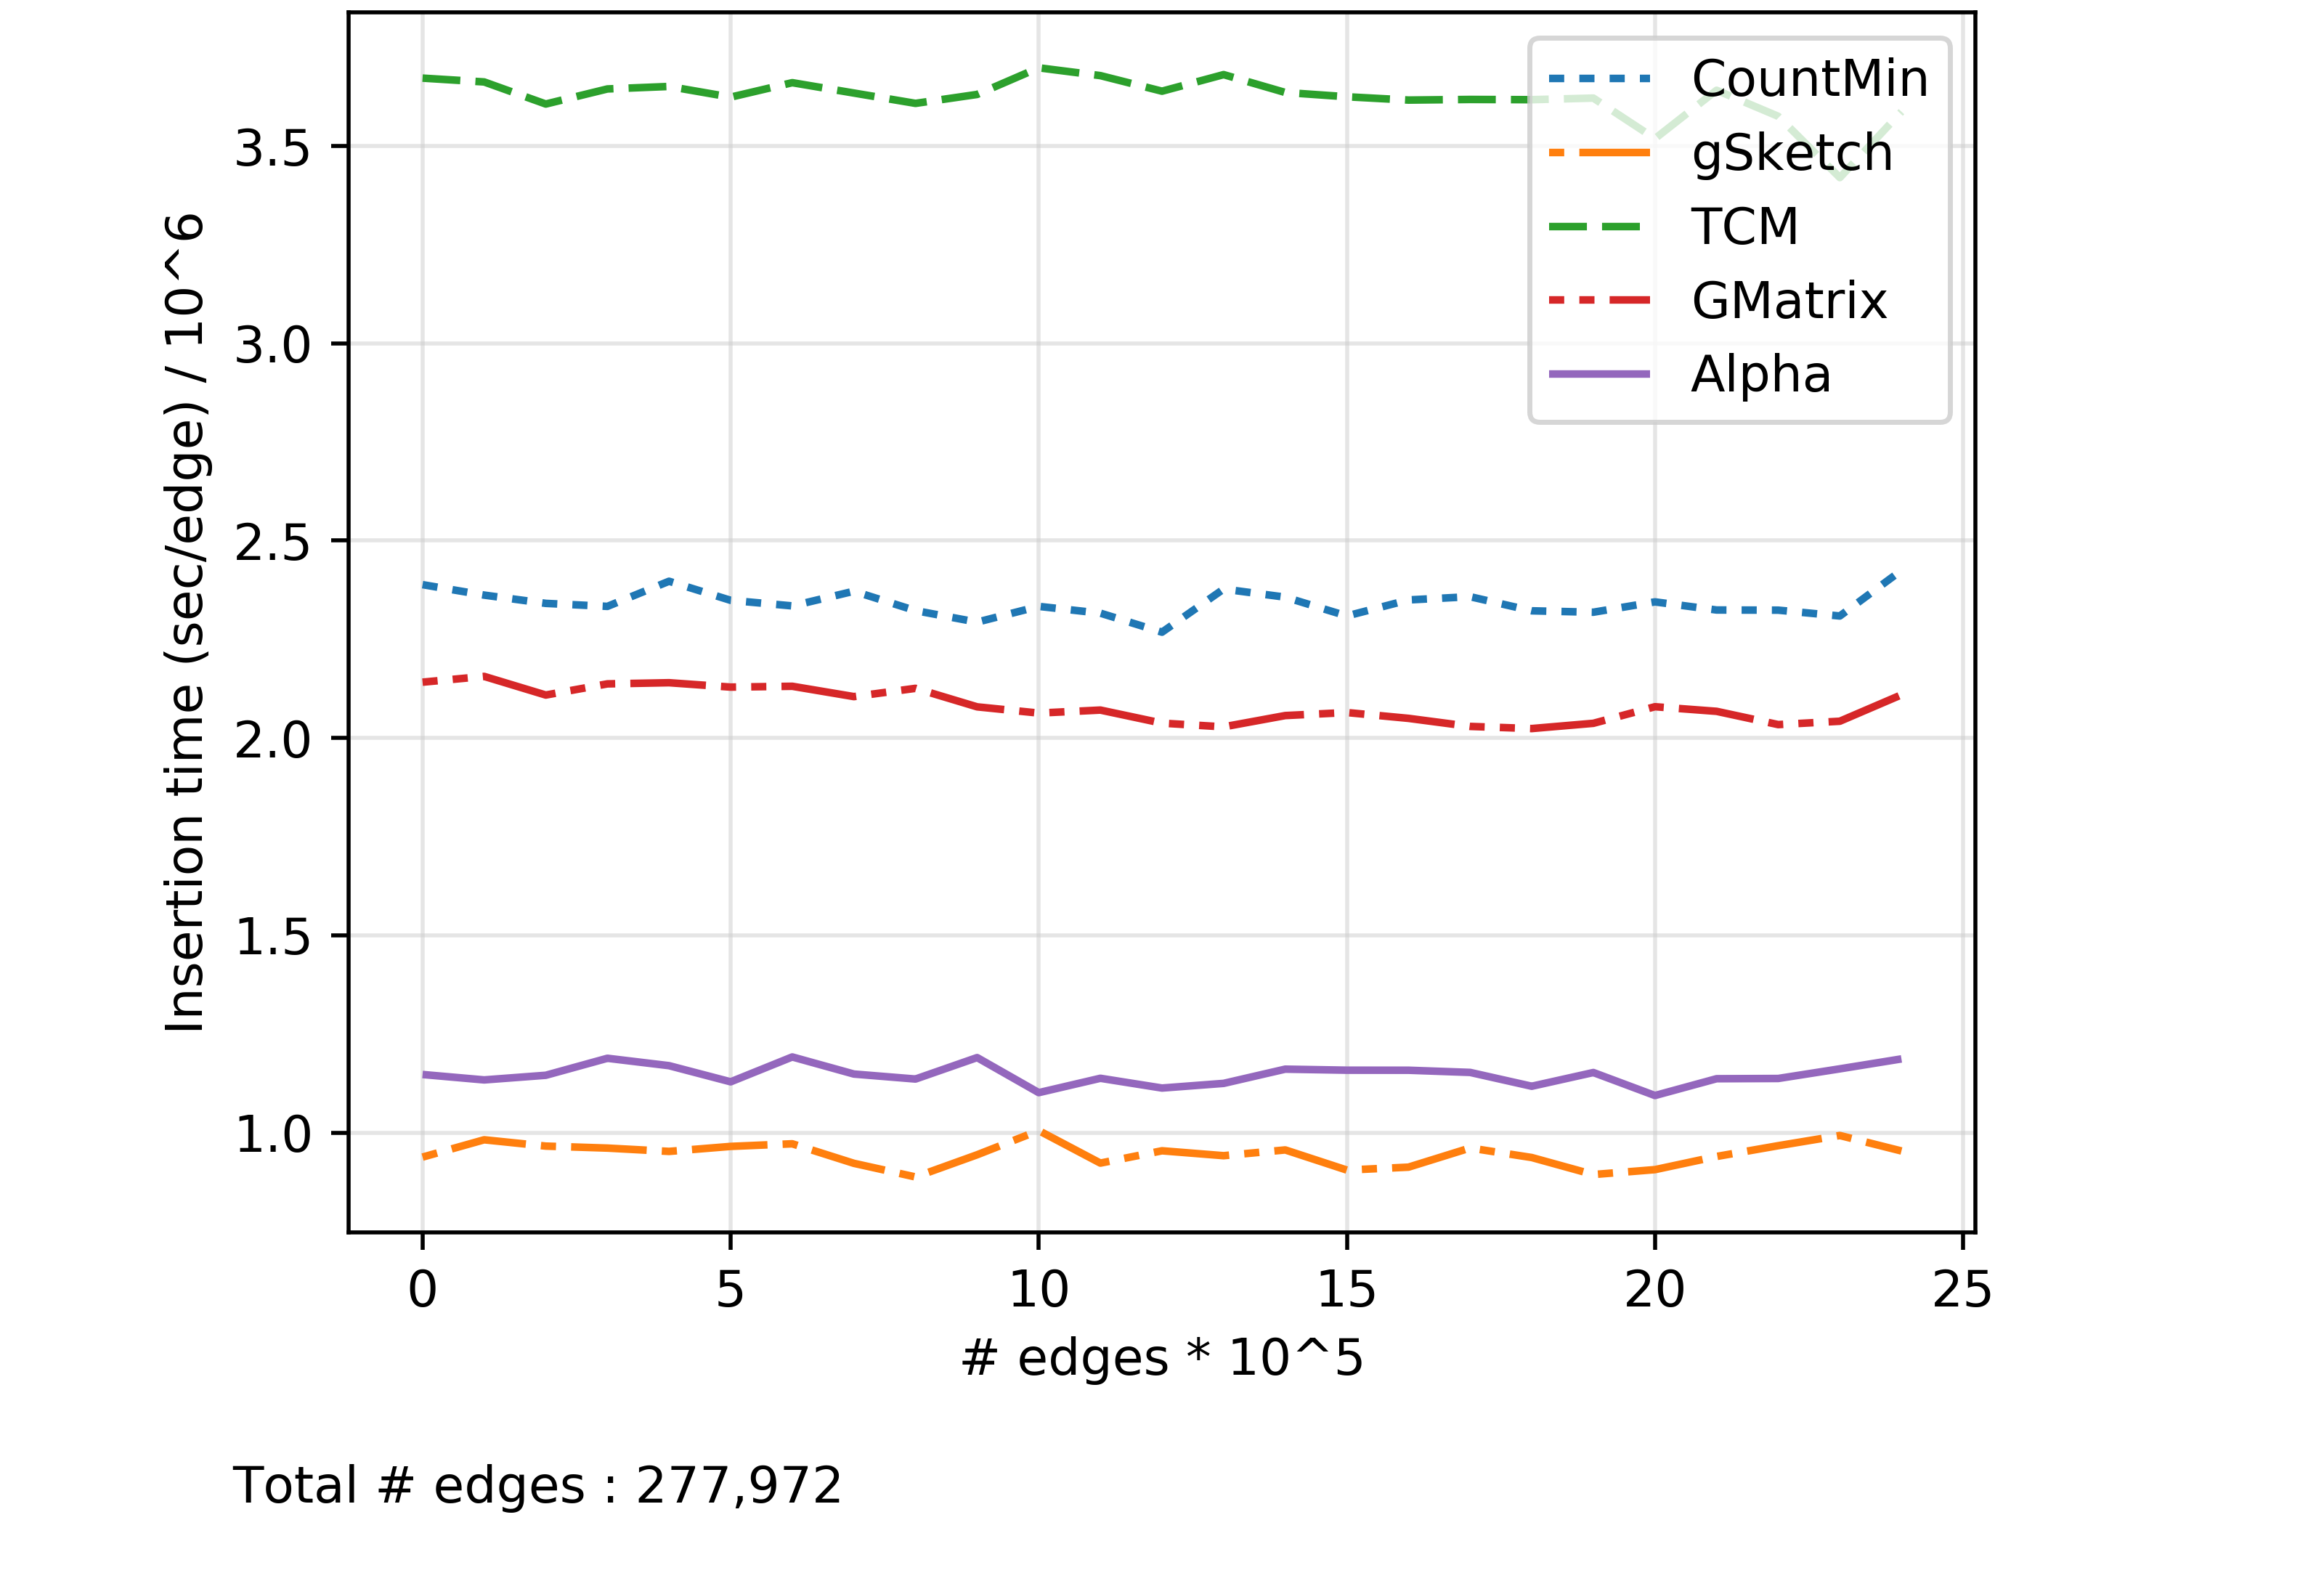
\includegraphics[width=0.85\textwidth]{results/insertion/unicorn-wget-insertiontime2_512}
    \vspace{-0.5cm}
    \caption{Insertion time per edge vs Number of edges in the sketch for unicorn-wget dataset}
    \label{fig:unicorn-wget-insertiontime2_512}
\end{figure}

\begin{figure}[H]
    \centering 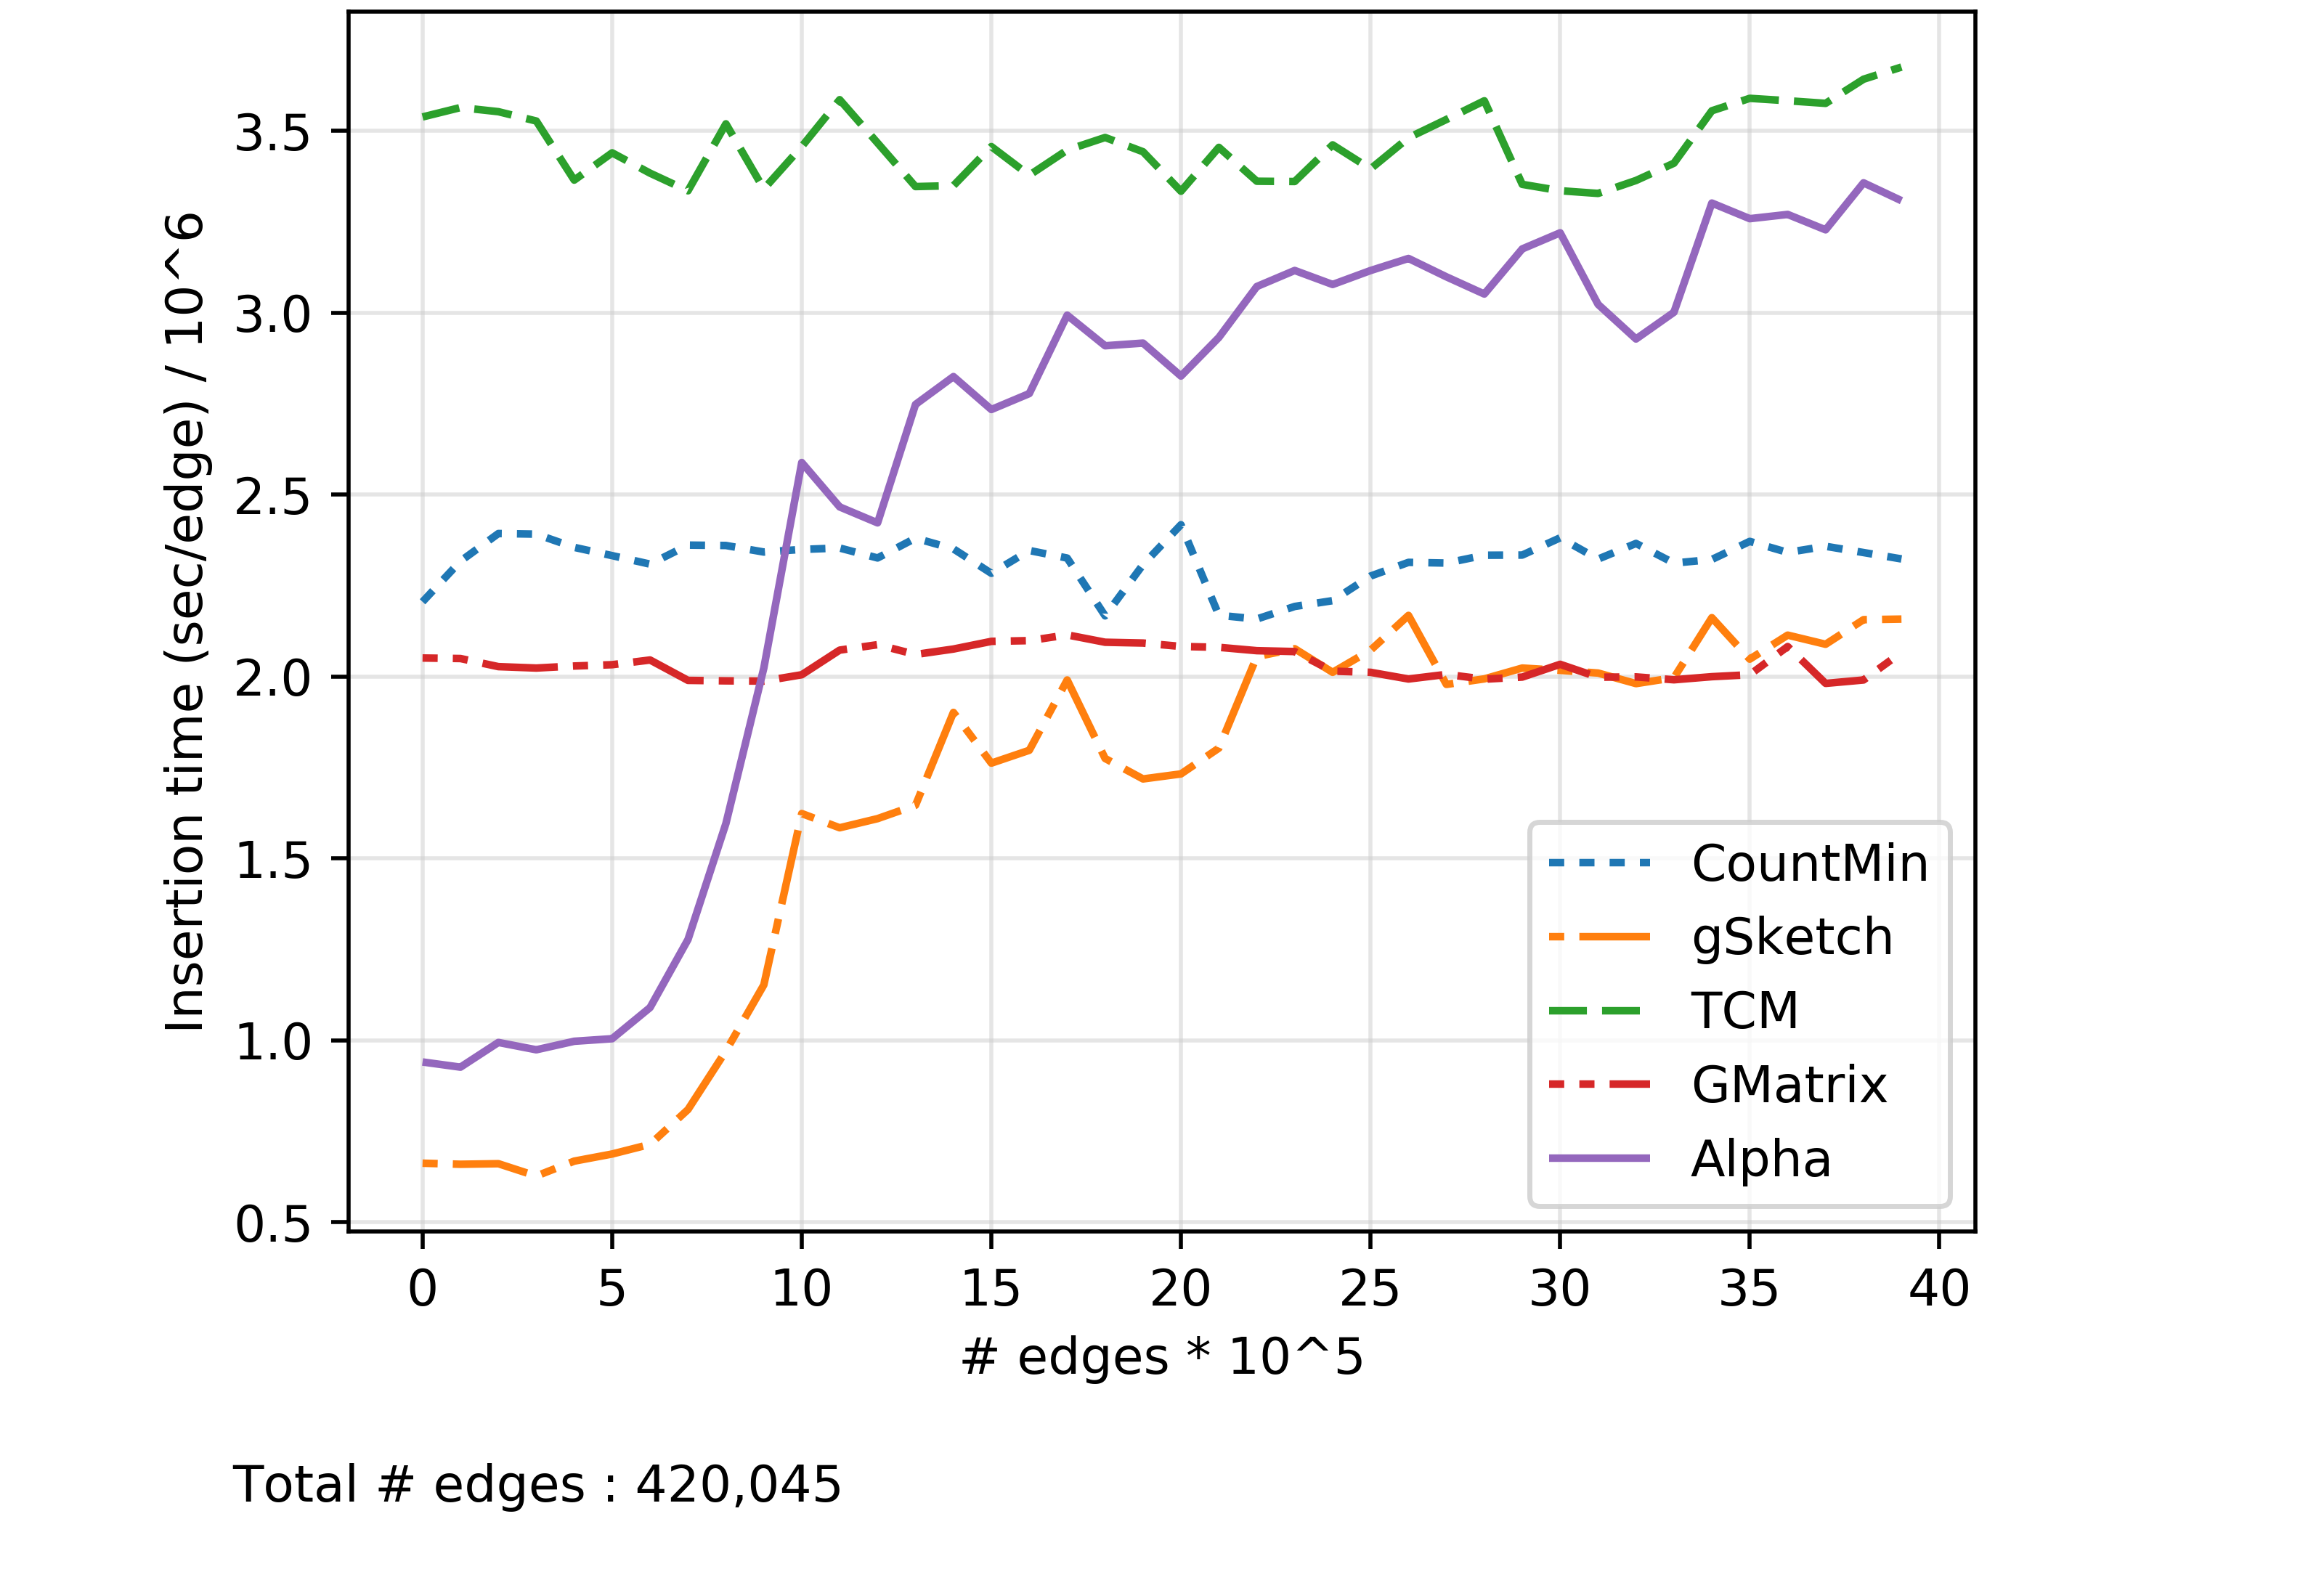
\includegraphics[width=0.85\textwidth]{results/insertion/email-EuAll-insertiontime2_512}
    \vspace{-0.5cm}
    \caption{Insertion time per edge vs Number of edges in the sketch for email-EuAll dataset}
    \label{fig:email-EuAll-insertiontime2_512}
\end{figure}

\begin{figure}[H]
    \centering 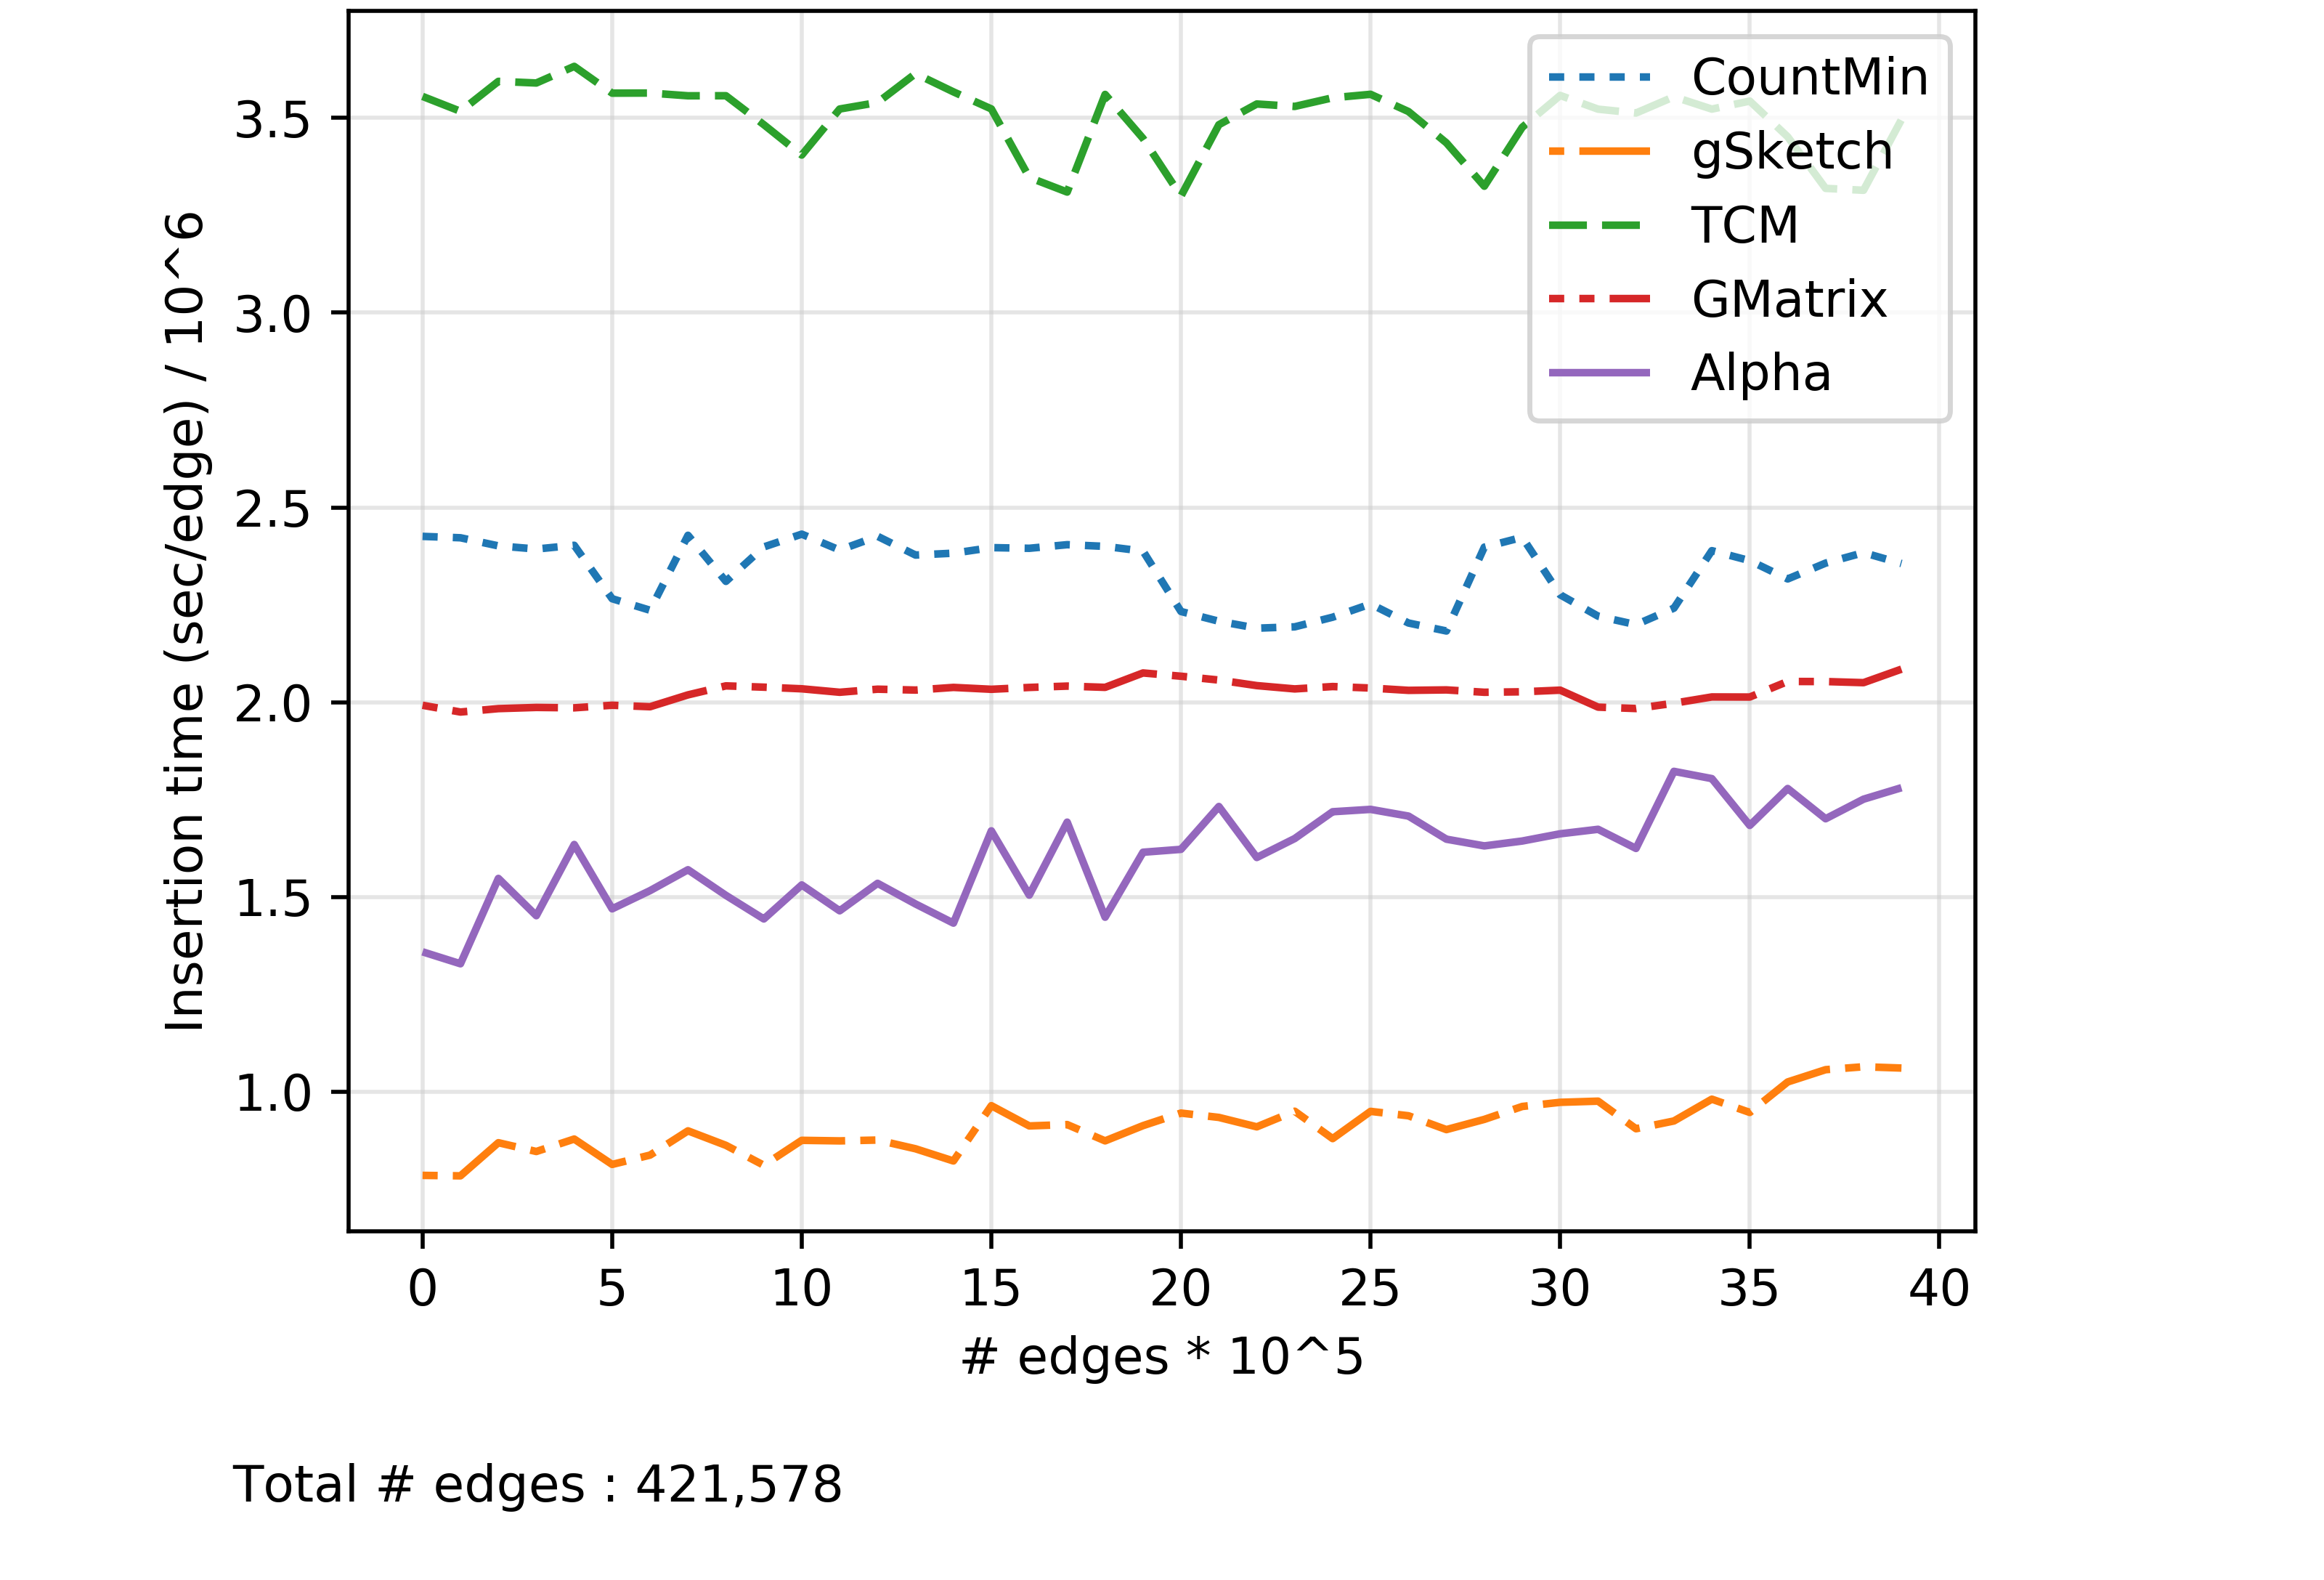
\includegraphics[width=0.85\textwidth]{results/insertion/cit-HepPh-insertiontime2_512}
    \vspace{-0.5cm}
    \caption{Insertion time per edge vs Number of edges in the sketch for cit-HepPh dataset}
    \label{fig:cit-HepPh-insertiontime2_512}
\end{figure}

\begin{figure}[H]
    \centering 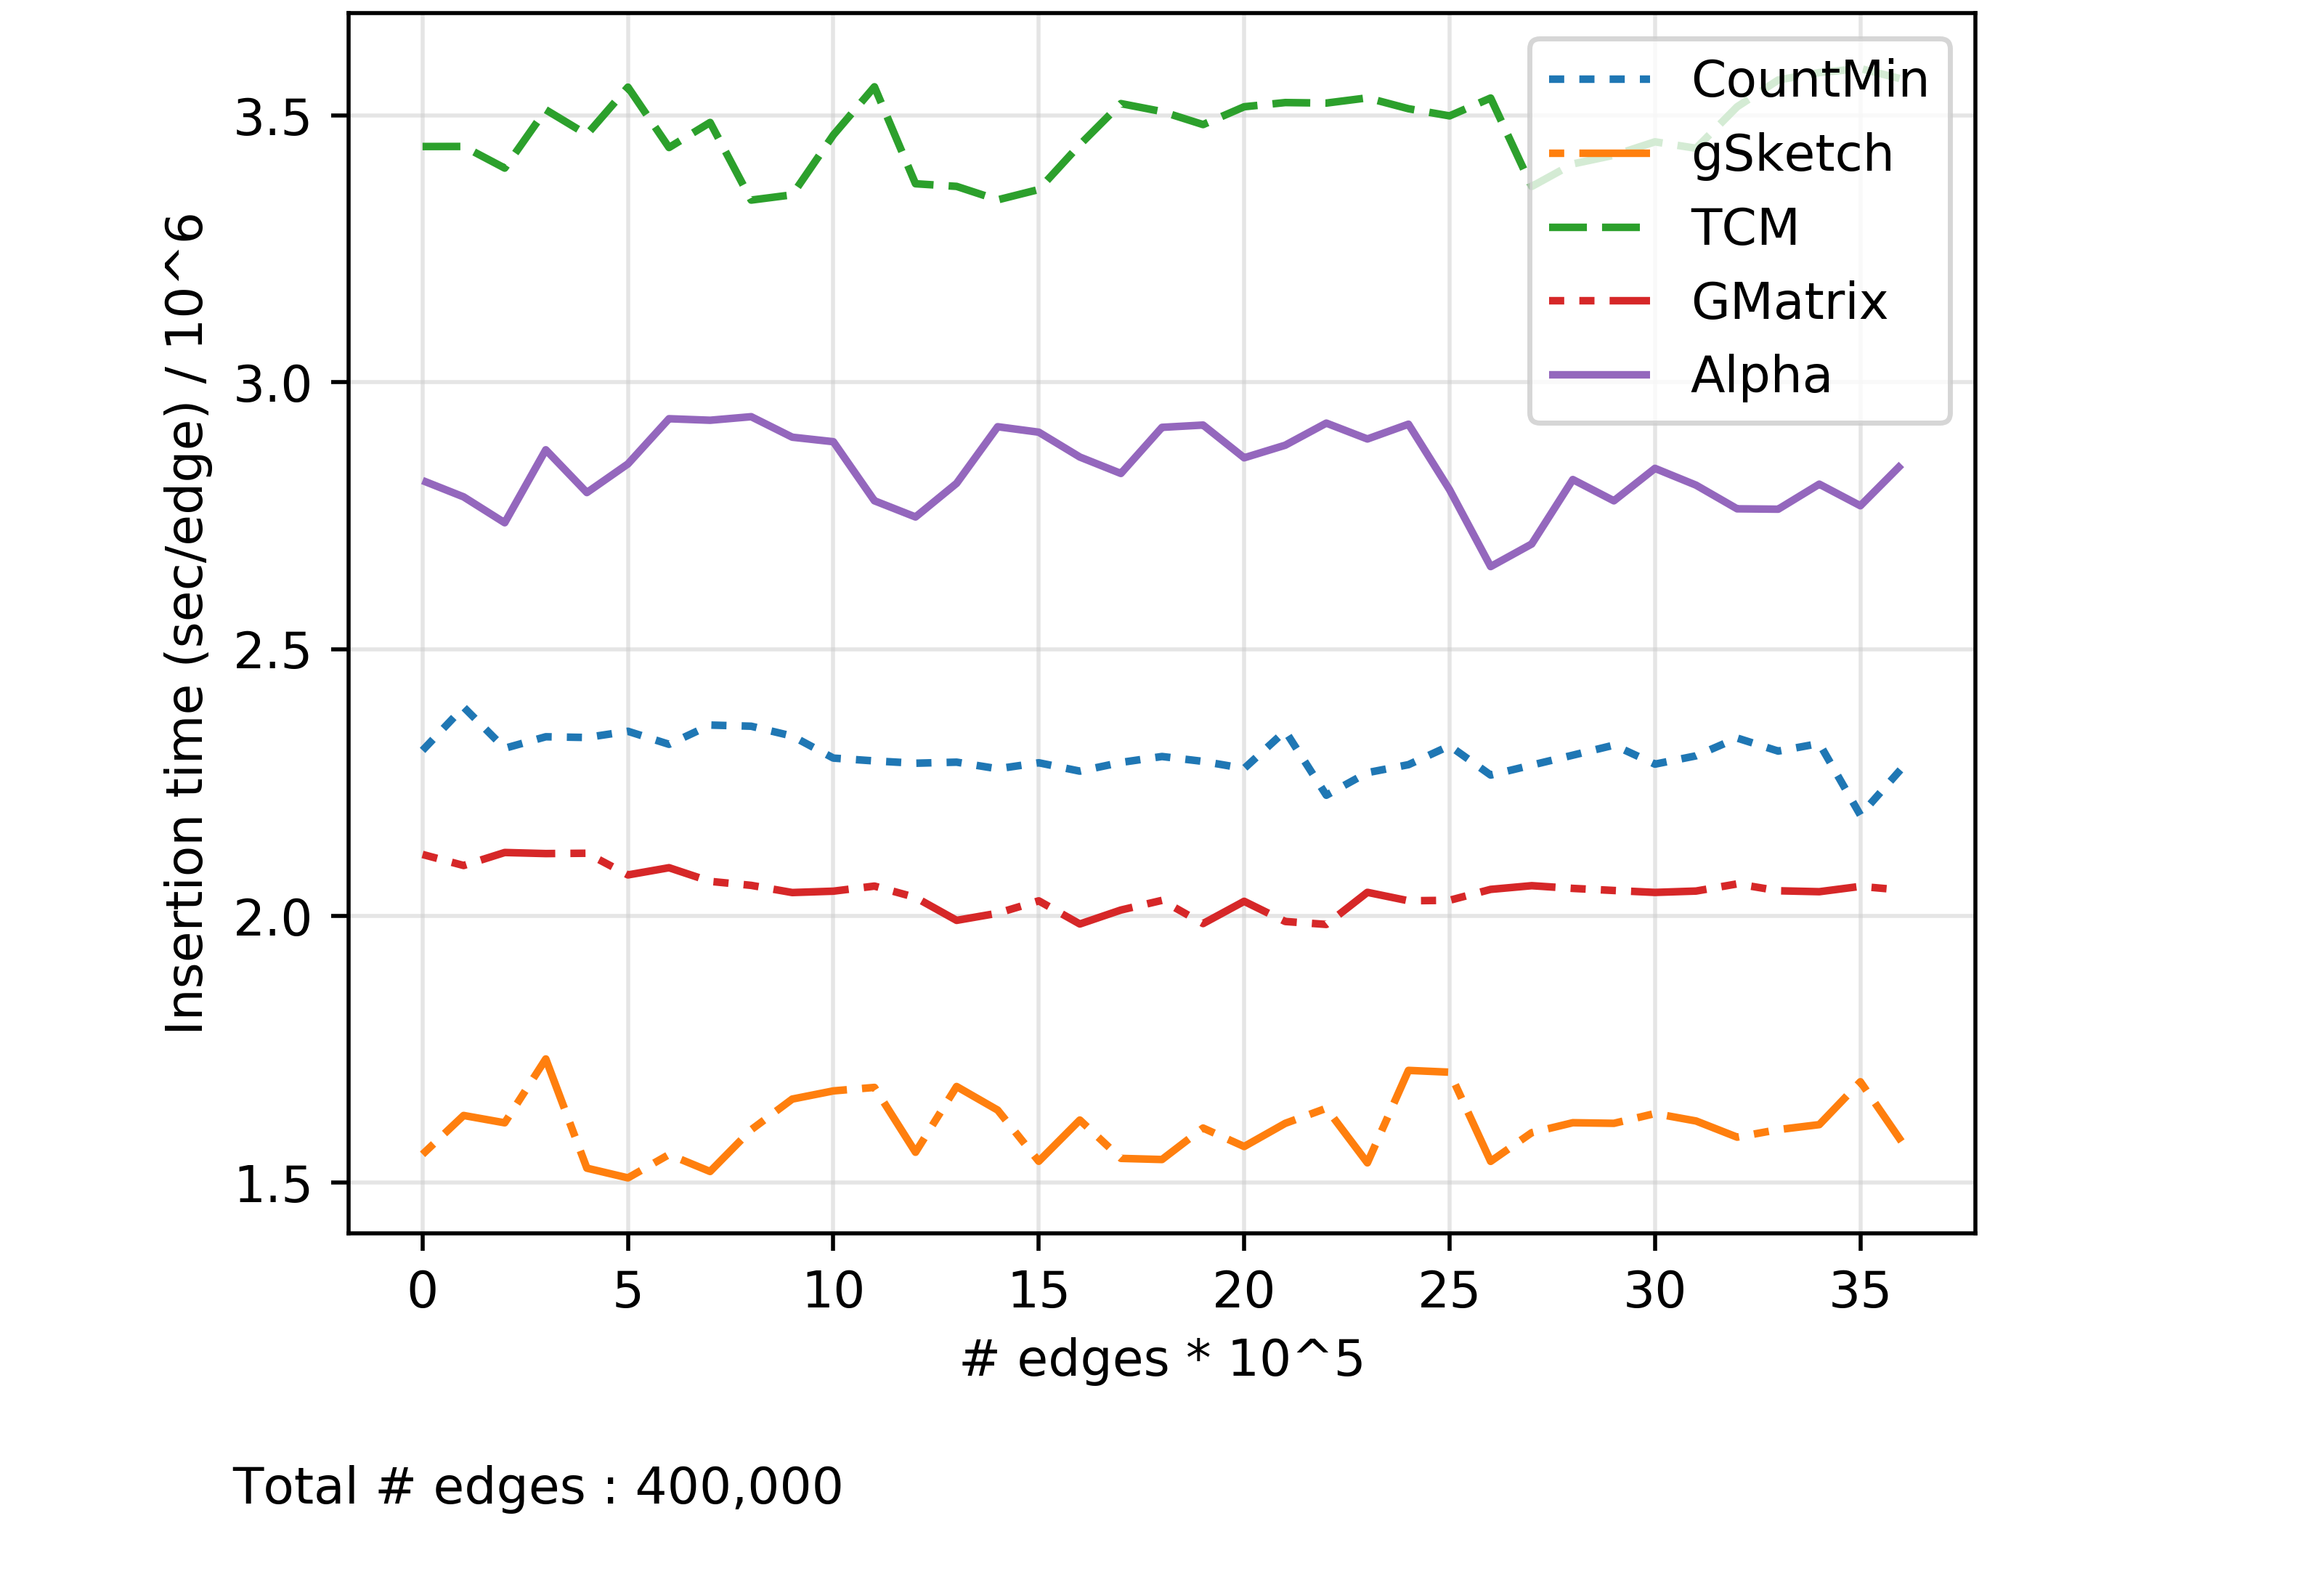
\includegraphics[width=0.85\textwidth]{results/insertion/gen-scale-free-insertiontime2_512}
    \vspace{-0.5cm}
    \caption{Insertion time per edge vs Number of edges in the sketch for gen-scale-free dataset}
    \label{fig:gen-scale-free-insertiontime2_512}
\end{figure}

\begin{figure}[H]
    \centering 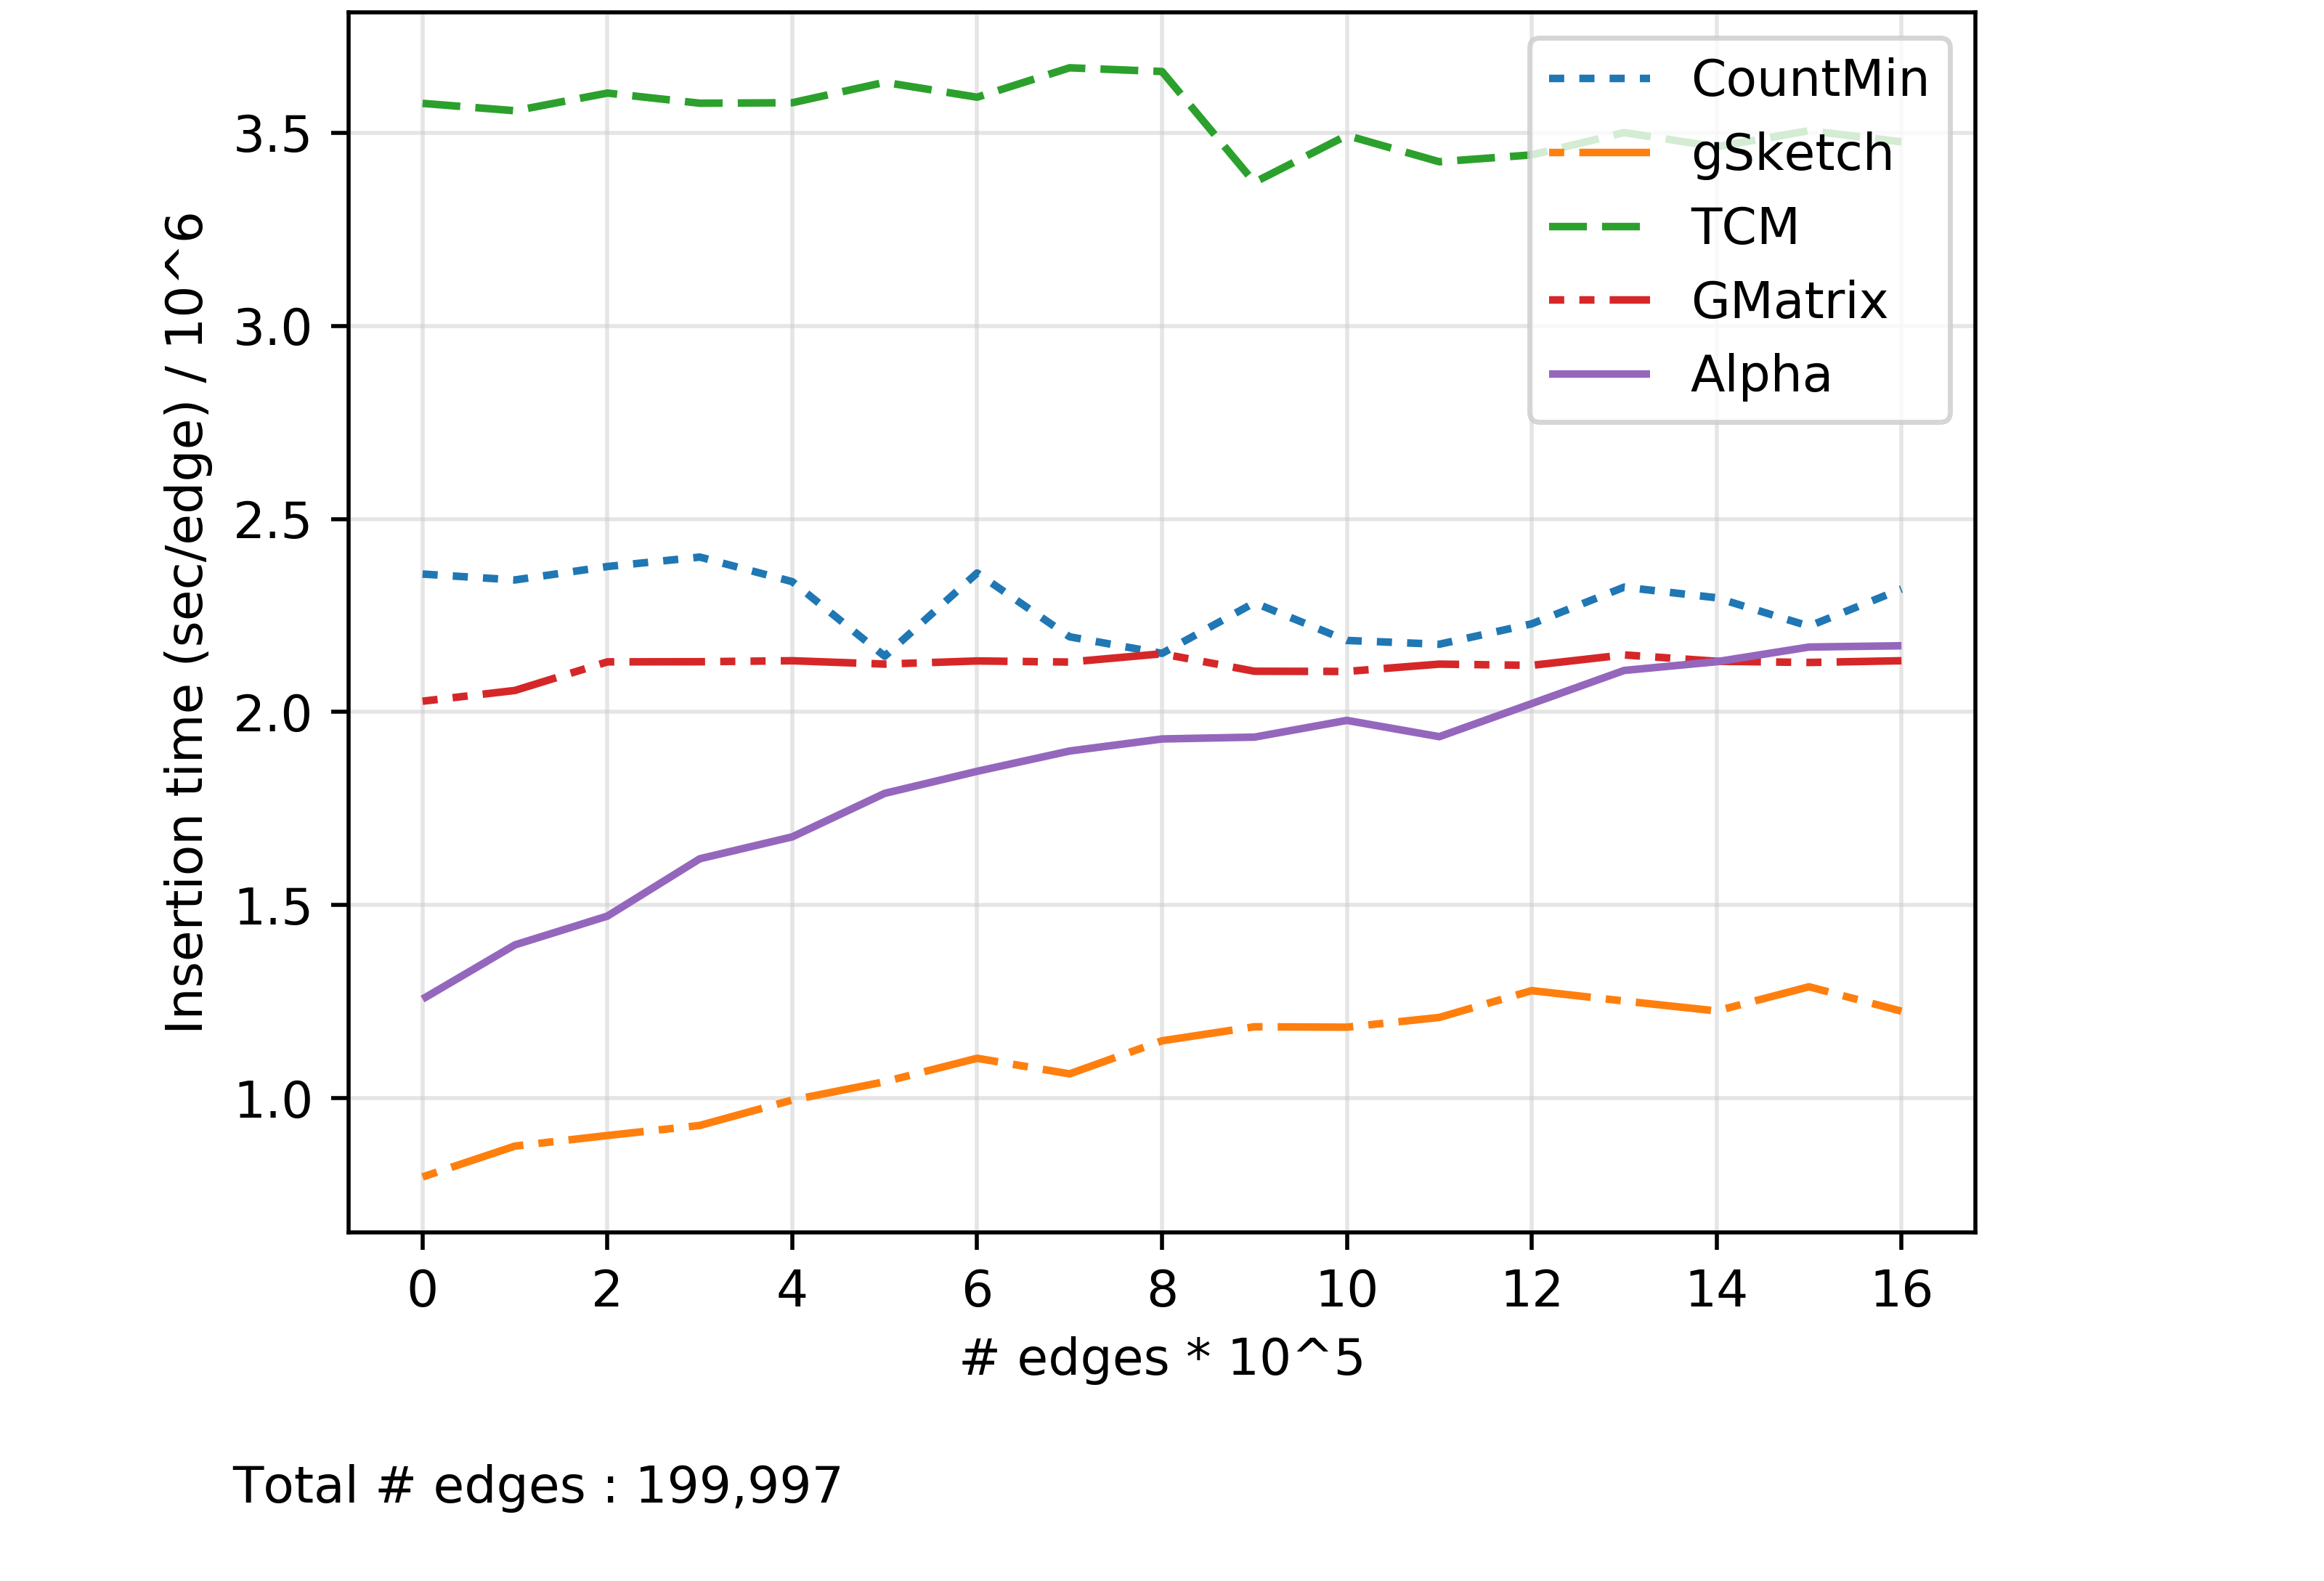
\includegraphics[width=0.85\textwidth]{results/insertion/gen-small-world-insertiontime2_512}
    \vspace{-0.5cm}
    \caption{Insertion time per edge vs Number of edges in the sketch for gen-small-world dataset}
    \label{fig:gen-small-world-insertiontime2_512}
\end{figure}

\subsubsection{Observations and inferences}

\paragraph{}
The speed of the edge operations (insertions) doesn't show a steady increase nor a decrease with respect to the amount of data in the sketch for the datasets depicted in \autoref{fig:unicorn-wget-insertiontime2_512}, \autoref{fig:cit-HepPh-insertiontime2_512}, \autoref{fig:gen-scale-free-insertiontime2_512} or \autoref{fig:gen-small-world-insertiontime2_512}.

\paragraph{}
\autoref{fig:email-EuAll-insertiontime2_512} of the dataset email-EuAll shows a steady increase of the insertion time per edge for the Alpha and gSketch sketches. We can infer that this is a result of the specific partitioning structure created for that particular dataset with the given parameters.

\paragraph{}
There is no direct correlation between the time per insertion operation and the number of edges present in the sketch. Thus we can conclude that there is no causation between the aforementioned properties as well.